% !Mode:: "TeX:UTF-8"
% !TEX program  = xelatex
\documentclass[a4paper]{article}
\usepackage{amsmath}
\usepackage{amssymb}
\usepackage{ctex}
\usepackage{graphicx}
\usepackage[european]{circuitikz}
\usepackage{multirow}
\usepackage{geometry}
\geometry{a4paper, top=2.54cm, bottom=2.54cm, left=2.54cm, right=2.54cm}
\title{三极管放大电路实验报告}
\author{王凯灵 521030910356}
\date{2022年11月20日}
\begin{document}
	\maketitle
	\section{实验目的}
	\begin{enumerate}
	\item 对三极管元件形成初步的认识, 学会使用三极管器件.
	\item 学习三级管放大电路的电路连接方法和工作原理, 学会根据需要调节三极管放大电路.
	\item 学会调节三极管电路的相关参数, 测量三极管电路的电路数据.
	\item 通过实验学习三极管放大电路的调试和故障分析.
	\end{enumerate}
	\section{实验仪器和原理}
	实验使用的三极管型号是9013, 实验使用的主要仪器有: 导线若干, DC电源, 通用示波器, 波形发生器, 万用表和JDEE-AD2II 实验箱, 上有电阻电容等电路元件和芯片若干. 
	
	9013三极管是一种小型NPN型管, 具有电路放大作用. 三极管具有三种工作状态: 放大, 截至, 饱和, 由$u_{be},u_{ce}$的大小关系决定. 三极管的输入输出图线如图所示.
	
	\begin{figure}[h]
		\begin{minipage}[t]{0.5\linewidth}
			\centering
			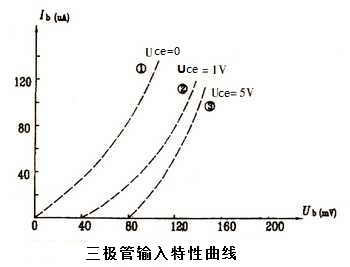
\includegraphics[width=0.8\linewidth]{输入}
			\caption{输入特性曲线}
		\end{minipage}
		\begin{minipage}[t]{0.5\linewidth}
			\centering
			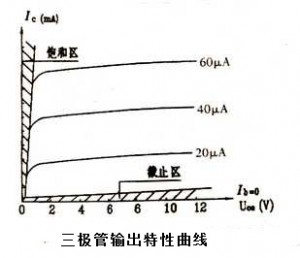
\includegraphics[width=0.8\linewidth]{输出}
			\caption{输出特性曲线}
		\end{minipage}		
	\end{figure}
	
	\begin{figure}[h]
		\centering
		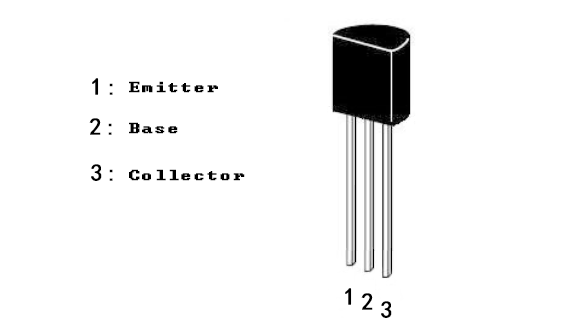
\includegraphics[width=0.5\linewidth]{9013三极管}
		\caption{9013三极管示意图}
	\end{figure}

	实验时, 主要采用共射放大电路, 其在实验箱上的电路图如图所示. 

	\begin{figure}[h]
		\begin{minipage}[t]{0.35\linewidth}
			\centering
			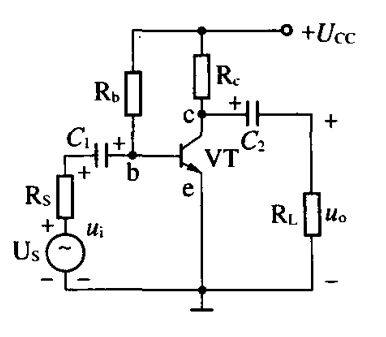
\includegraphics[width=0.9\linewidth]{原理图}
			\caption{原理图}
		\end{minipage}
		\begin{minipage}[t]{0.65\linewidth}
			\centering
			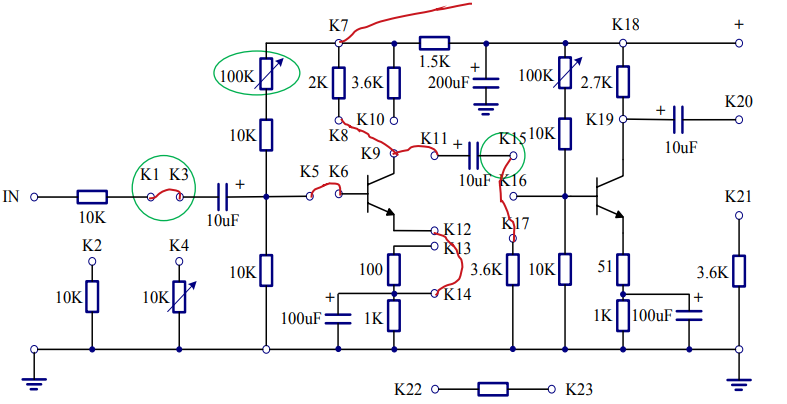
\includegraphics[width=0.9\linewidth]{电路图}
			\caption{电路图}
		\end{minipage}		
	\end{figure}

	分析放大电路的一般方法是: 1)作出直流通路得到静态工作点. 2)作出动态电路分析放大性能. 
	
	\section{实验过程与结果}
	
	\subsection{静态电路分析}
	实际使用+9V Vcc正确连接电路如图所示, 作出直流通路图. 通过微调滑动变阻器调节基极电压$U_B = 2.25V$. 测量数据如表1所示. 
	
	\begin{figure}[h]
		\centering
		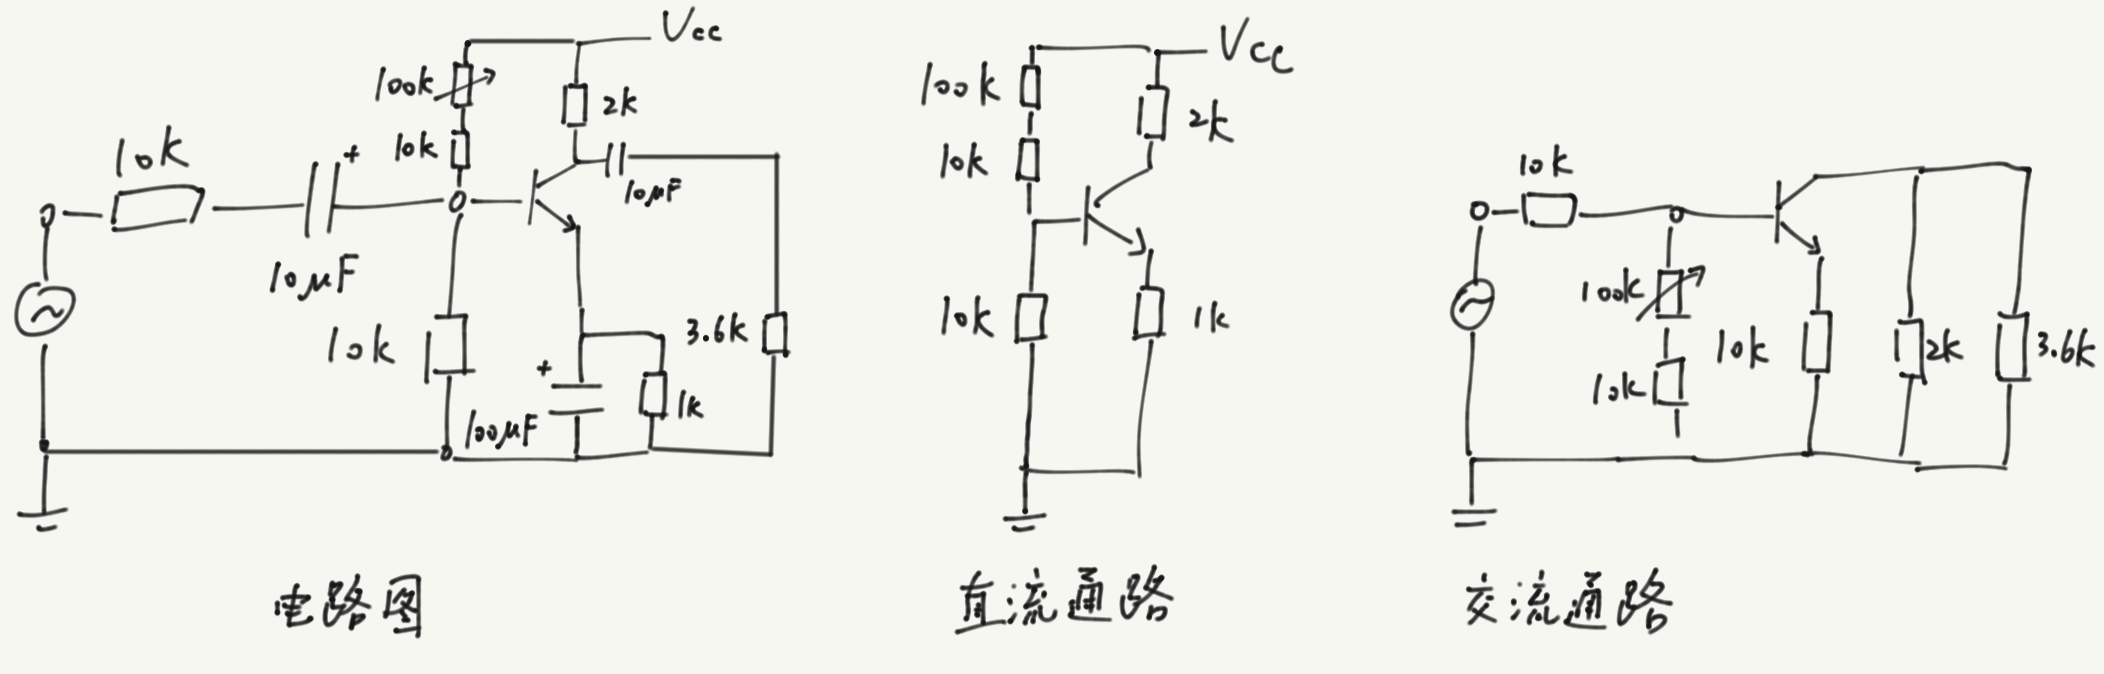
\includegraphics[width=0.9\linewidth]{绘图}
		\caption{手绘电路图, 直流通路, 交流通路}
	\end{figure}

	\begin{figure}[h]
		\begin{minipage}[t]{0.5\linewidth}
			\centering
			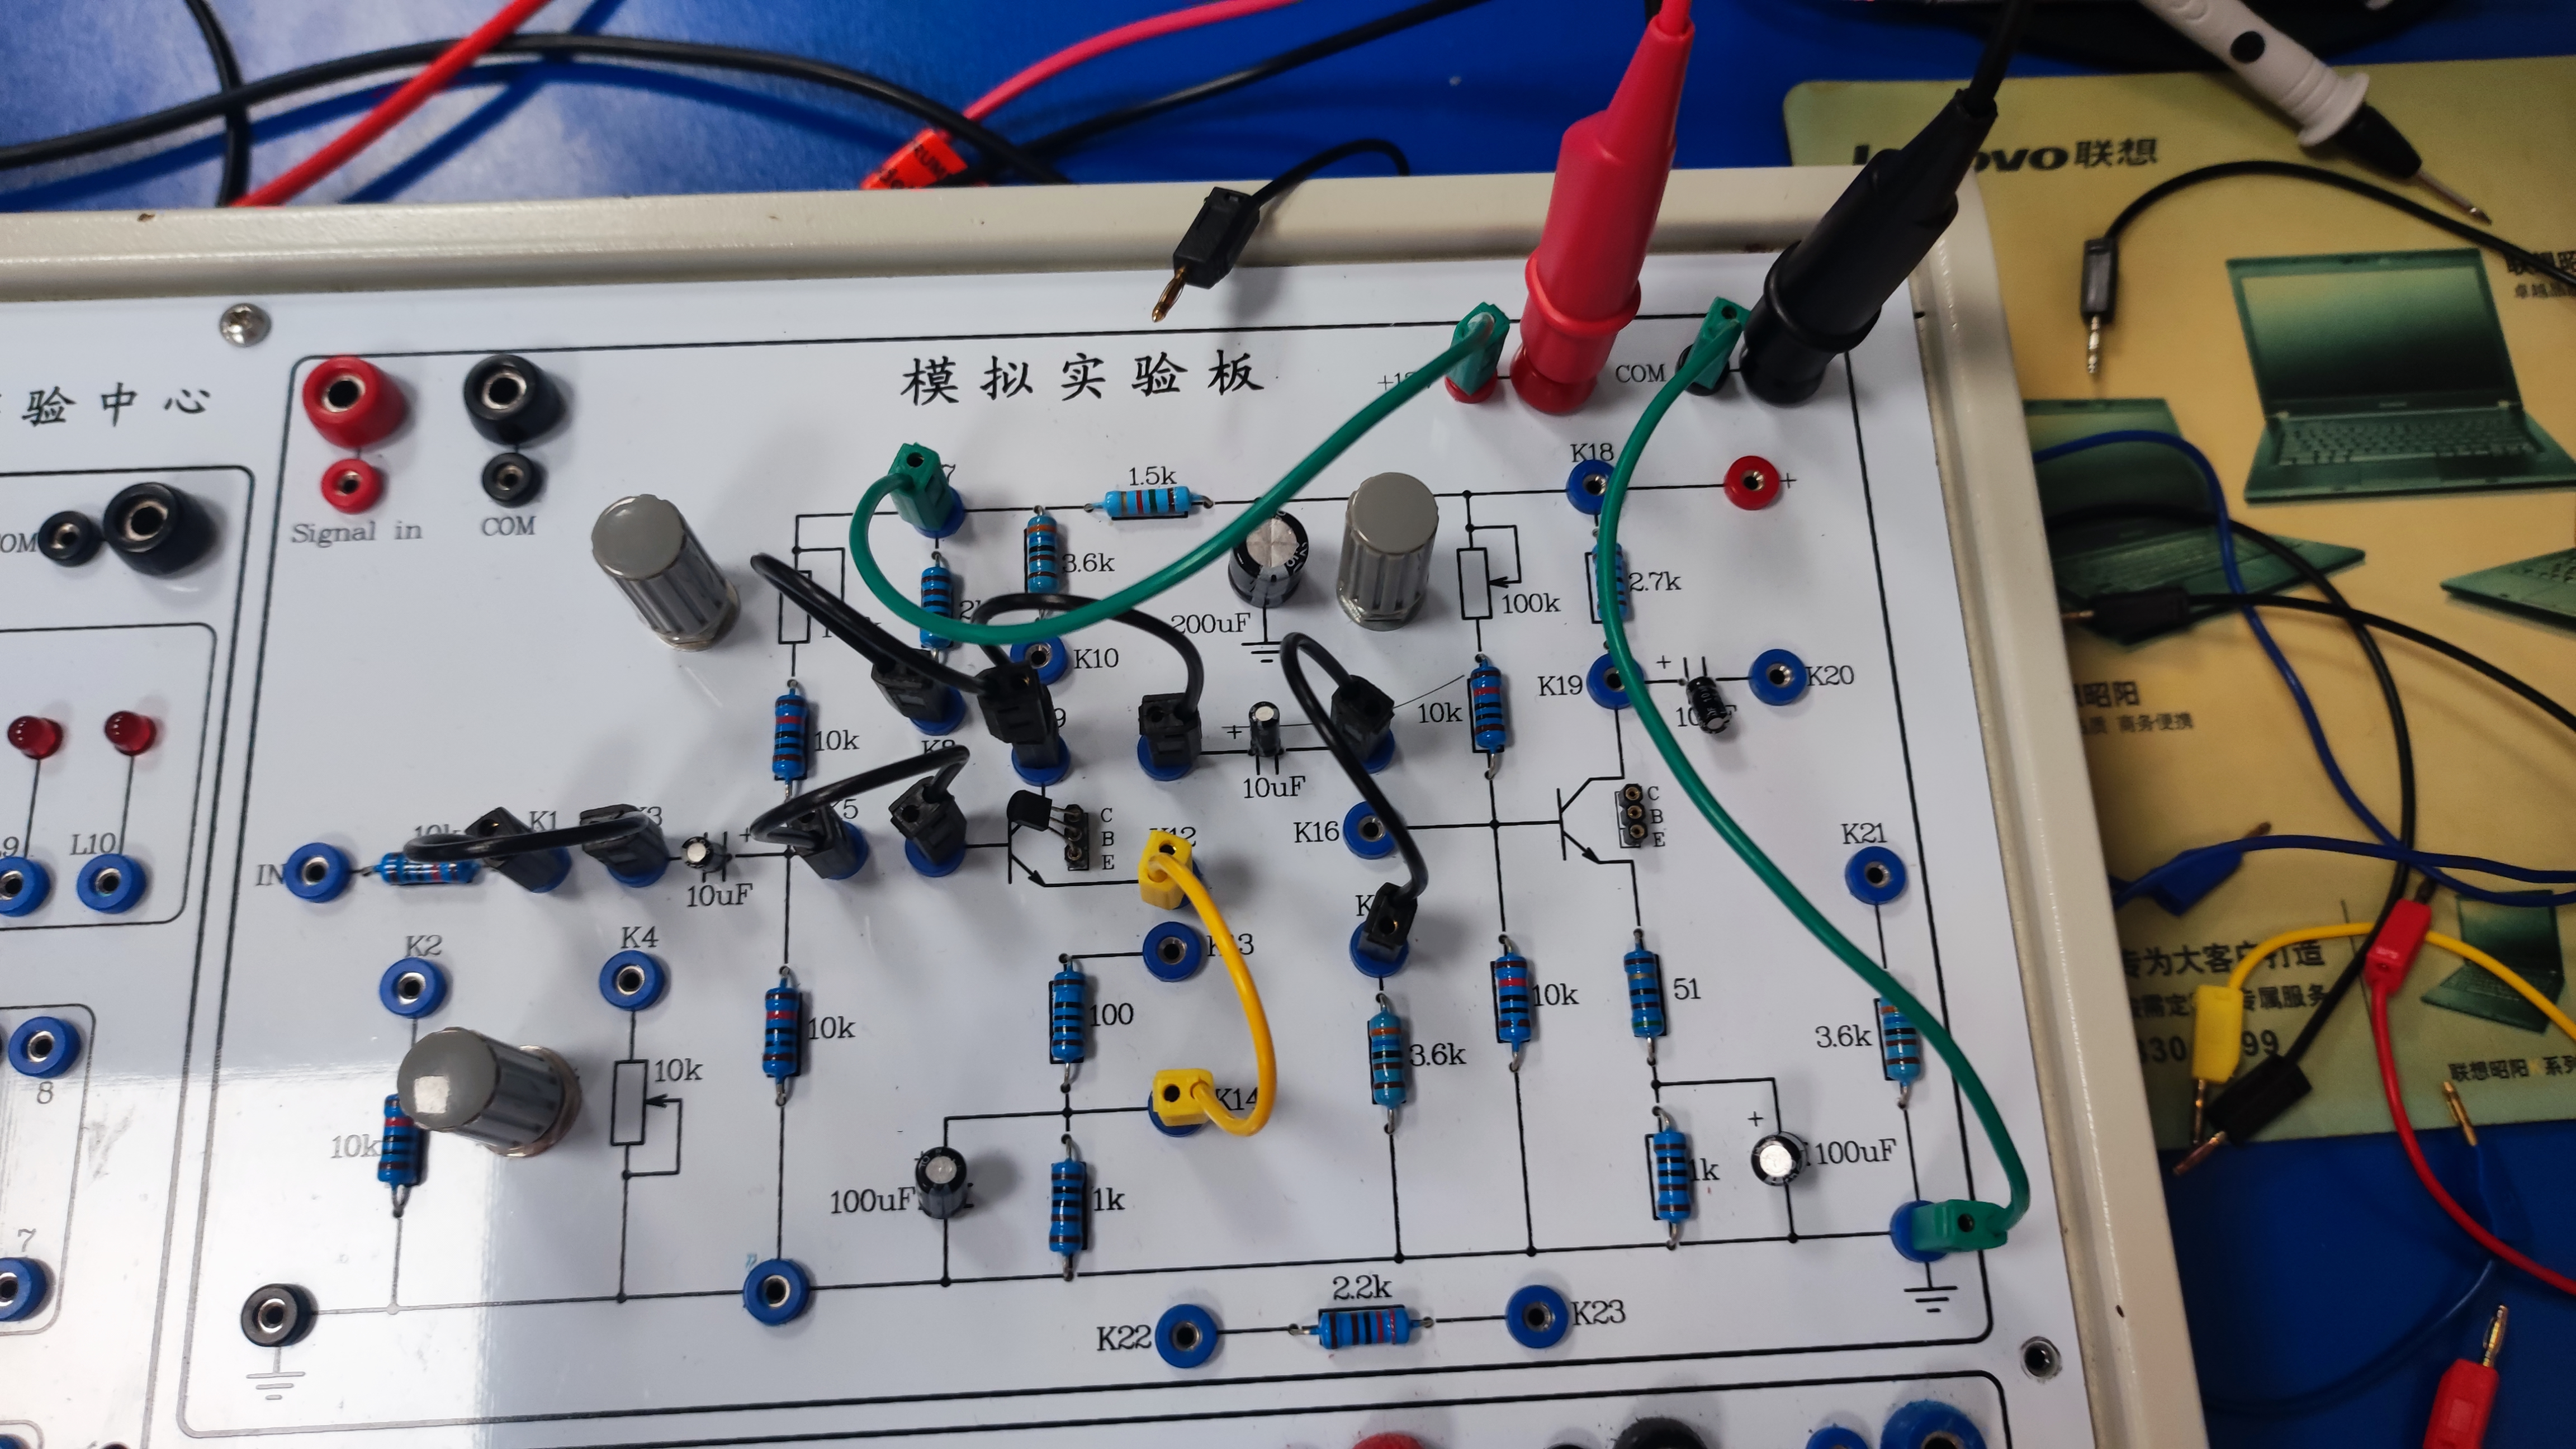
\includegraphics[width=0.9\linewidth]{图片/静态工作}
			\caption{静态工作实物图}
		\end{minipage}
		\begin{minipage}[t]{0.5\linewidth}
			\centering
			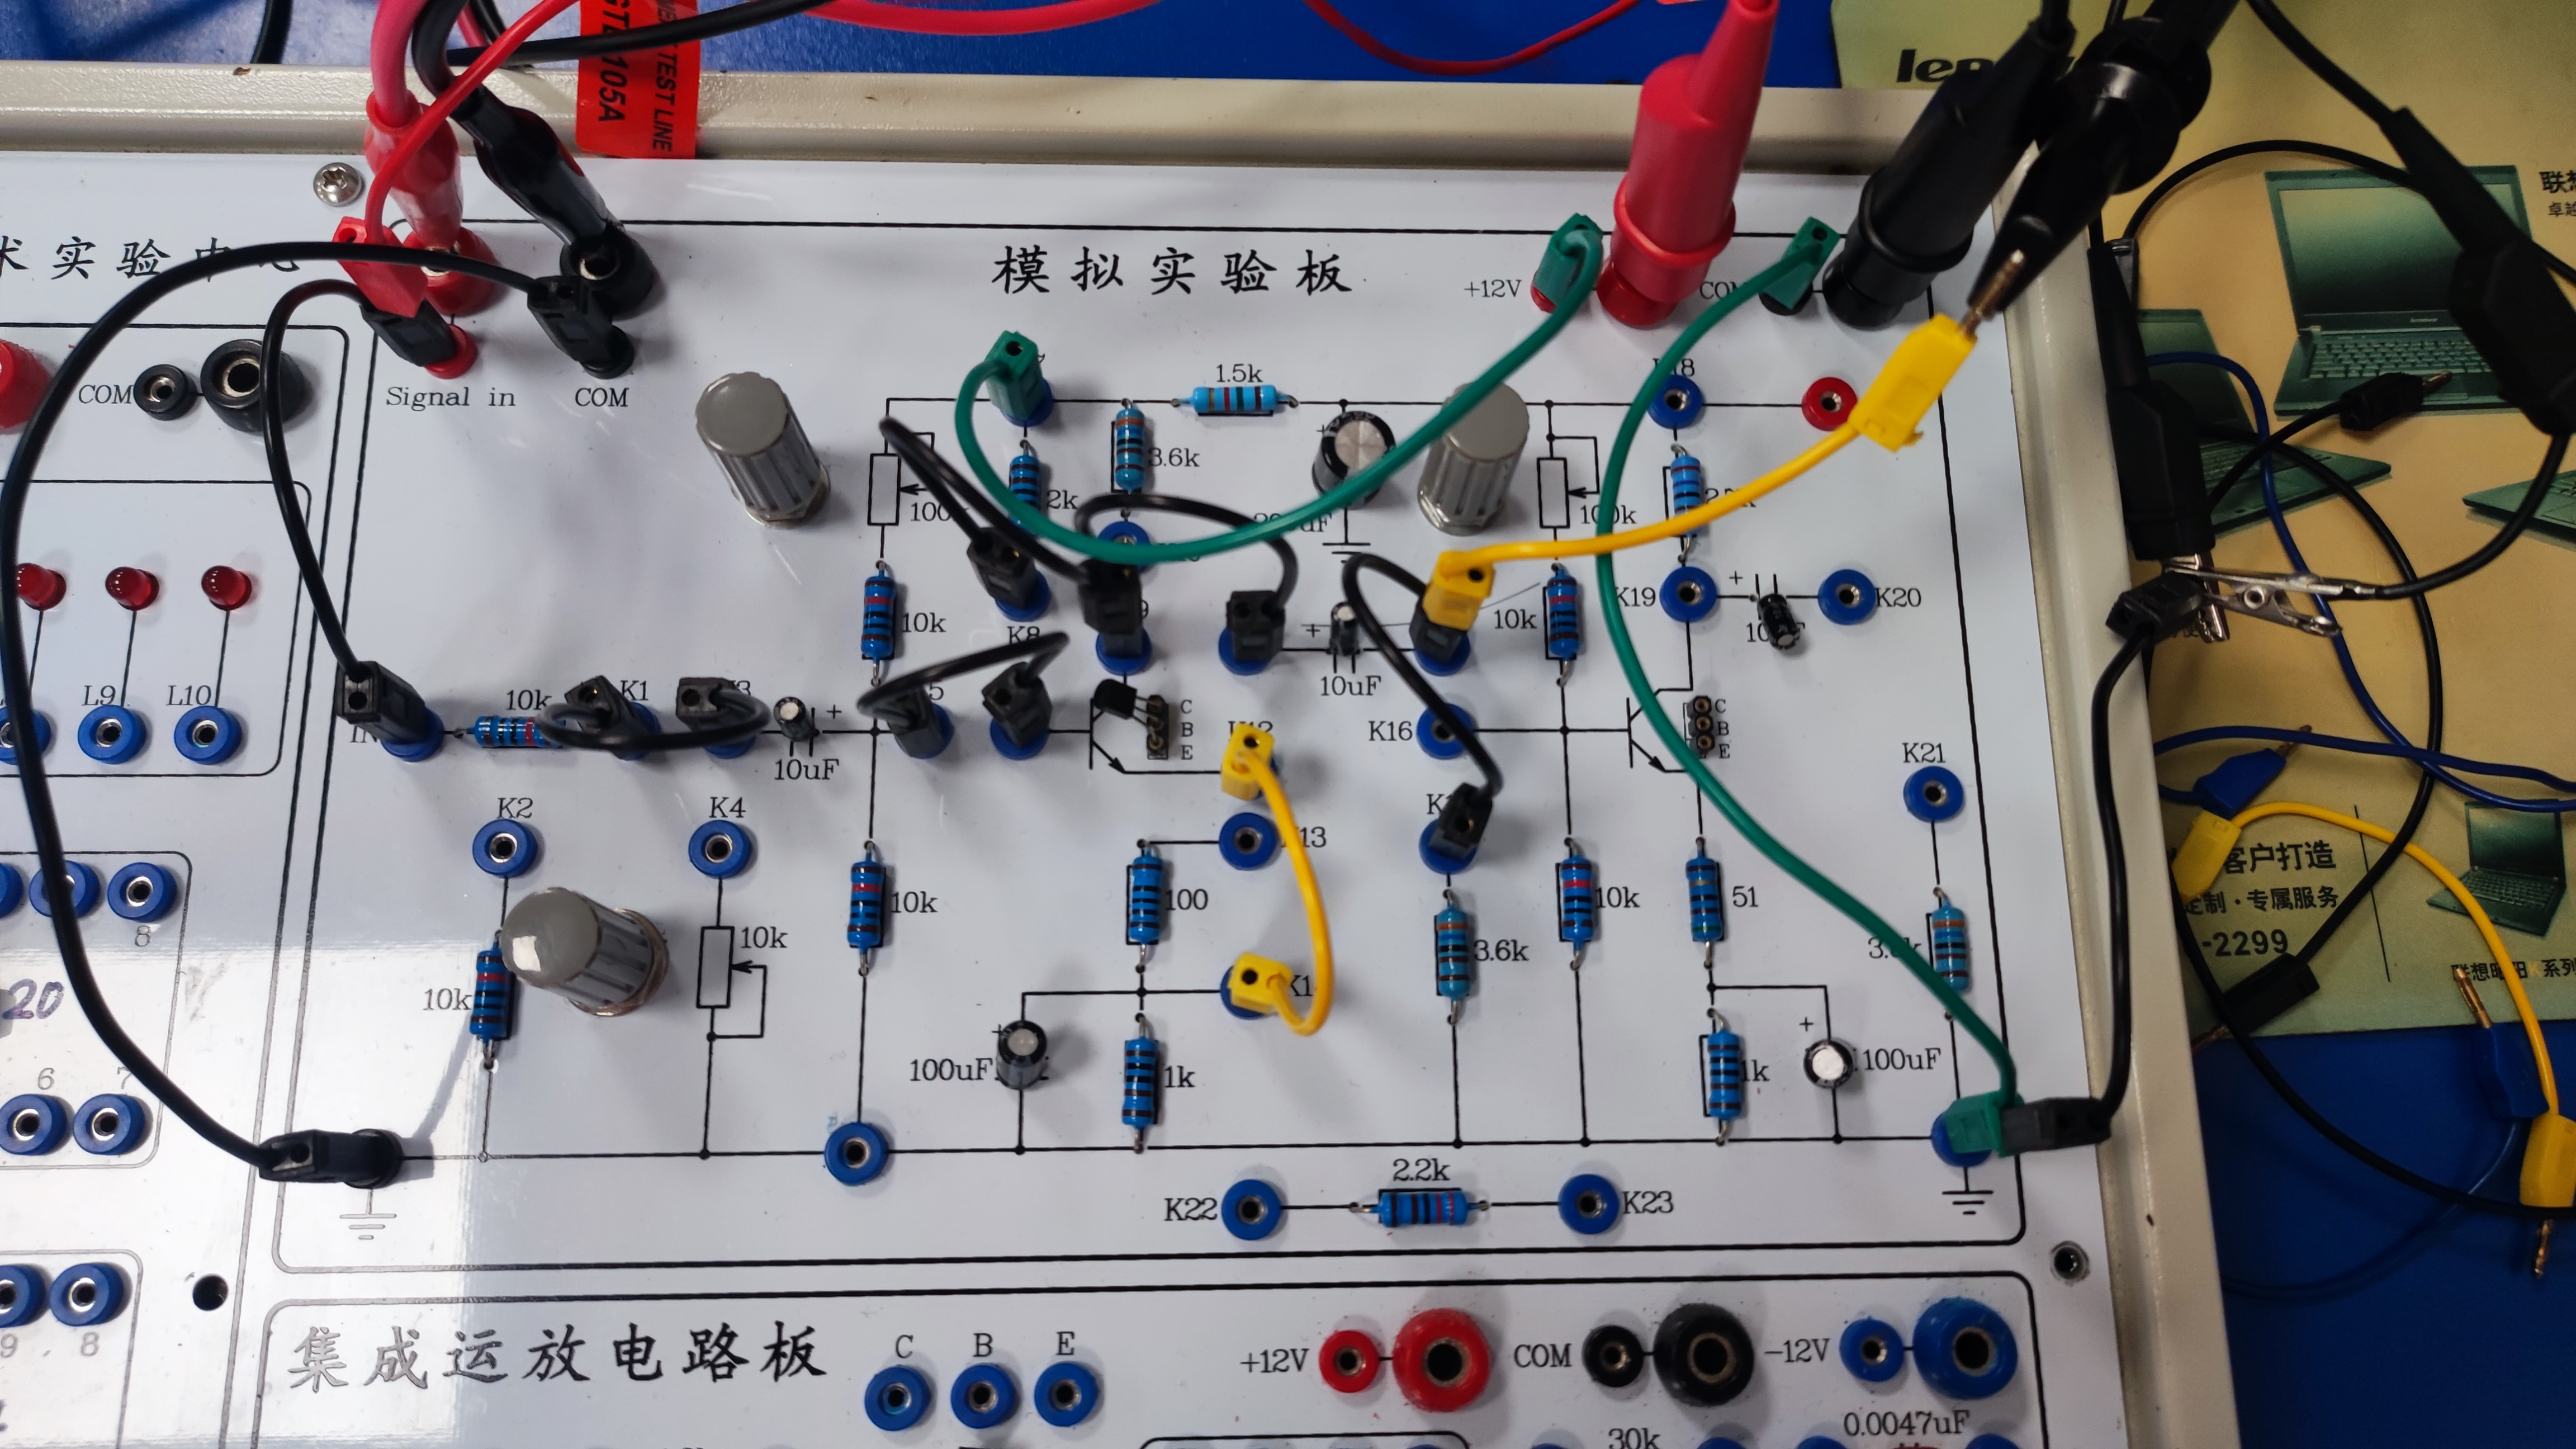
\includegraphics[width=0.9\linewidth]{图片/外加交流}
			\caption{动态电路实物图}
		\end{minipage}		
	\end{figure}
	
	\begin{table}[h]
		\centering
		\caption{静态电路数据}
		\begin{tabular}{l|l|l|l|l}
			\hline
			 & $U_B/V$ & $U_C/V$ & $U_E/V$ & $U_{CE}/V$ \\ \hline
			正确连接电路时 & 2.25 & 5.78 & 1.62 & 4.15 \\ \hline
			K5-K6之间的连线断开 & 0.00 & 8.99 & 0.00 & 8.99 \\ \hline
			K8-K9之间的连线断开 & 2.85 & 0.198 & 0.197 & -0.001 \\ \hline
			K7-K8之间的电阻短路 & 2.25 & 8.99 & 1.57 & 7.41 \\ \hline
		\end{tabular}
	\end{table}
	
	正确连接电路时, 电路处于放大区, 工作正常. 此时$U_B-U_E=U_{BEQ}\approx 0.63V$. $U_{CQ}>U_{BQ}>U_{EQ}$.
	
	当K5, K6断开时, $U_B=U_E=0, U_C\approx Vcc$, 因为基极电路开路, 可认为电位为0, 则三极管工作在截至区, $I_{BEQ}=0$. 故集电极电位为Vcc. 
	
	当K8, K9断开时, 集电极开路反偏, 三极管不正常工作. 此时基极电压来自于Vcc分压, $U_C\approx U_E=U_B-U_{BEQ}$. 
	
	当K7, K8短路时, Vcc短接集电极. 故$U_C\approx Vcc$, 由于三极管处于放大区, $U_B=U_{BQ}, U_E=U_{EQ}$. 但电路不具有放大功能, 因为$U_{CE}$无法变化. 
	
	由测量数据, 估算$I_{C Q}=\frac{Vcc-U_{CQ}}{R_C}=1.61mA, I{E Q}=\frac{U_{EQ}}{R_E}=1.62mA$. 
	
	由静态工作点计算公式, 
	
	$$
	\begin{aligned}
		I_{B Q} &=\frac{V_{C C}-U_{B E Q}}{R_B} \\
		& \approx \frac{V_{C C}-0.62}{R_B} \approx \frac{V_{C C}}{R_B} \\ 
		I_{C Q} &= \beta I_{B Q}
	\end{aligned}
	$$
	
	发现测量的精度不够, 无法根据静态工作点的测量计算放大倍数. 
	
	\section{动态电路分析}
	调整好静态工作点后, 如上图所示, 连接动态电路. 接入200mVpp的正弦信号, 示波器观察输入输出.
	 
	在空载时, 输出信号大约为3.16Vpp, 输入信号测量值为216mVpp, 输入信号大小为35mVpp. 波形也未失真, 此时电压放大倍数为$\frac{U_o}{U_i}\approx101.1$	
	
	在负载时, 输出信号大约为2.16Vpp. 信号源测量值为220mVpp, 输入信号大小为35mVpp. 波形均为发生失真现象, 三极管放大电路工作正常. 此时的电压放大倍数为$\frac{U_o}{U_i}\approx61.71$. 
	
	\begin{figure}[h]
		\begin{minipage}[t]{0.5\linewidth}
			\centering
			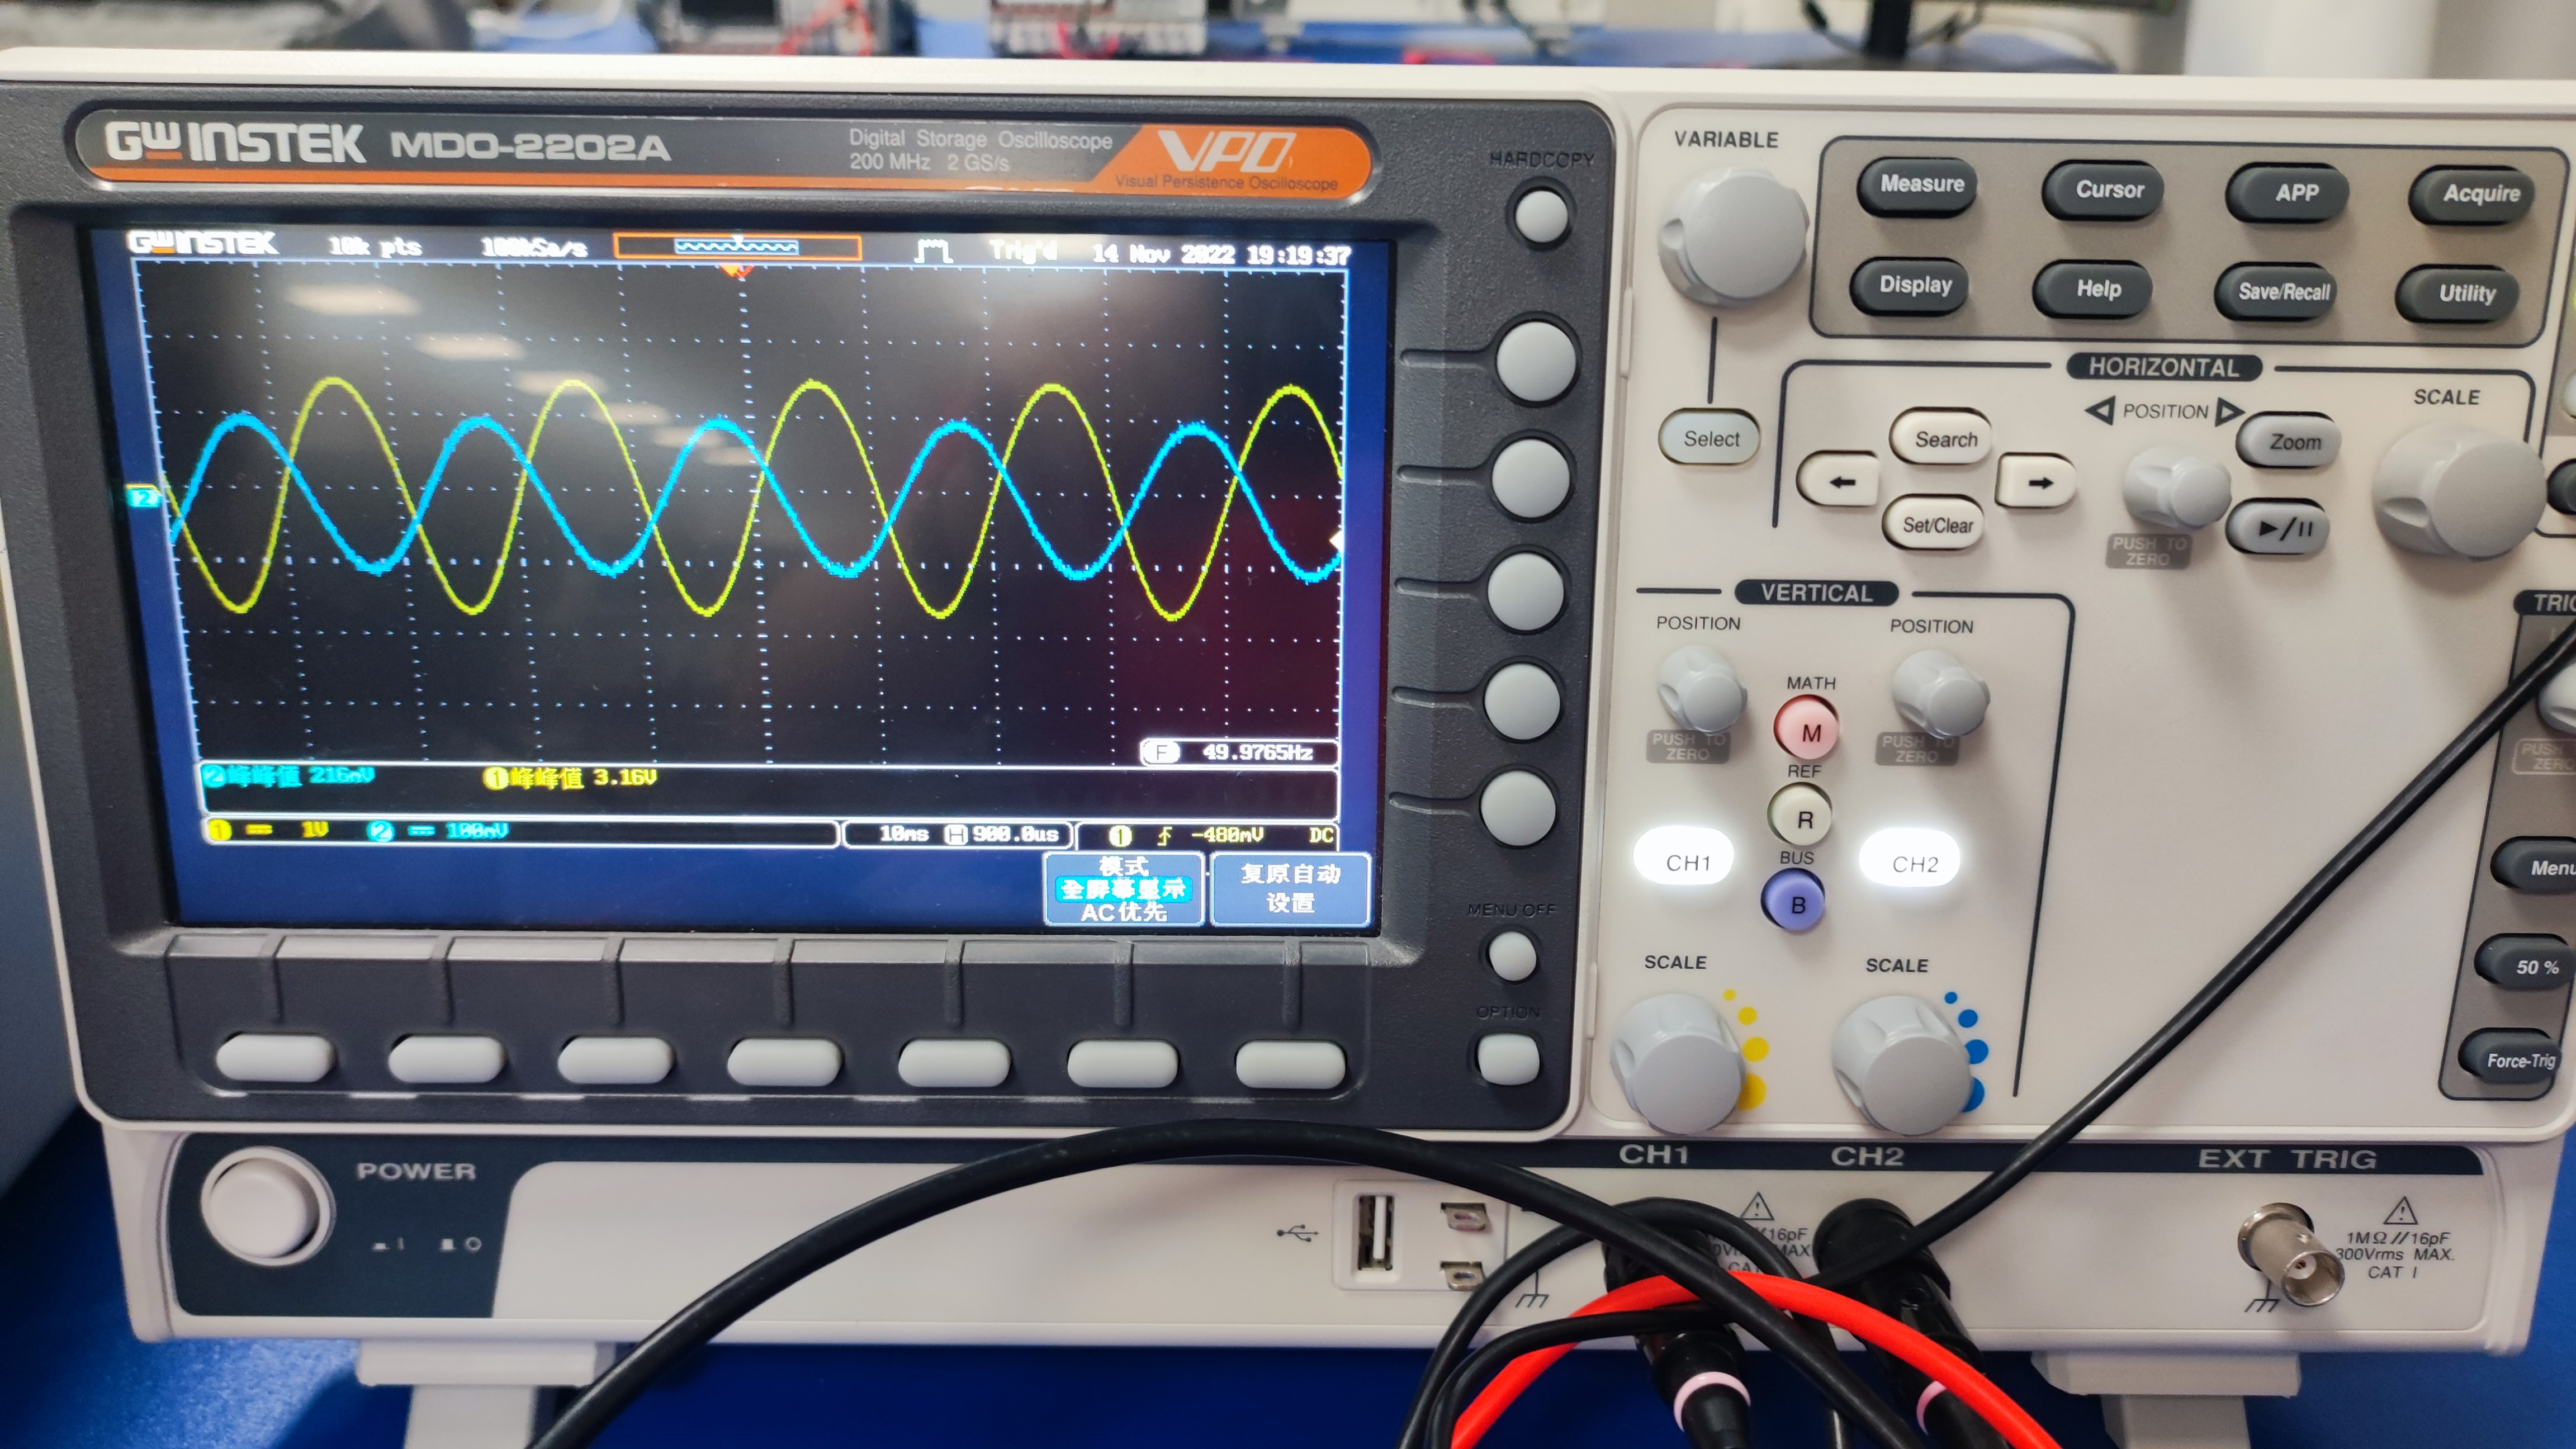
\includegraphics[width=0.9\linewidth]{图片/负载放大}
			\caption{空载放大示波器}
		\end{minipage}
		\begin{minipage}[t]{0.5\linewidth}
			\centering
			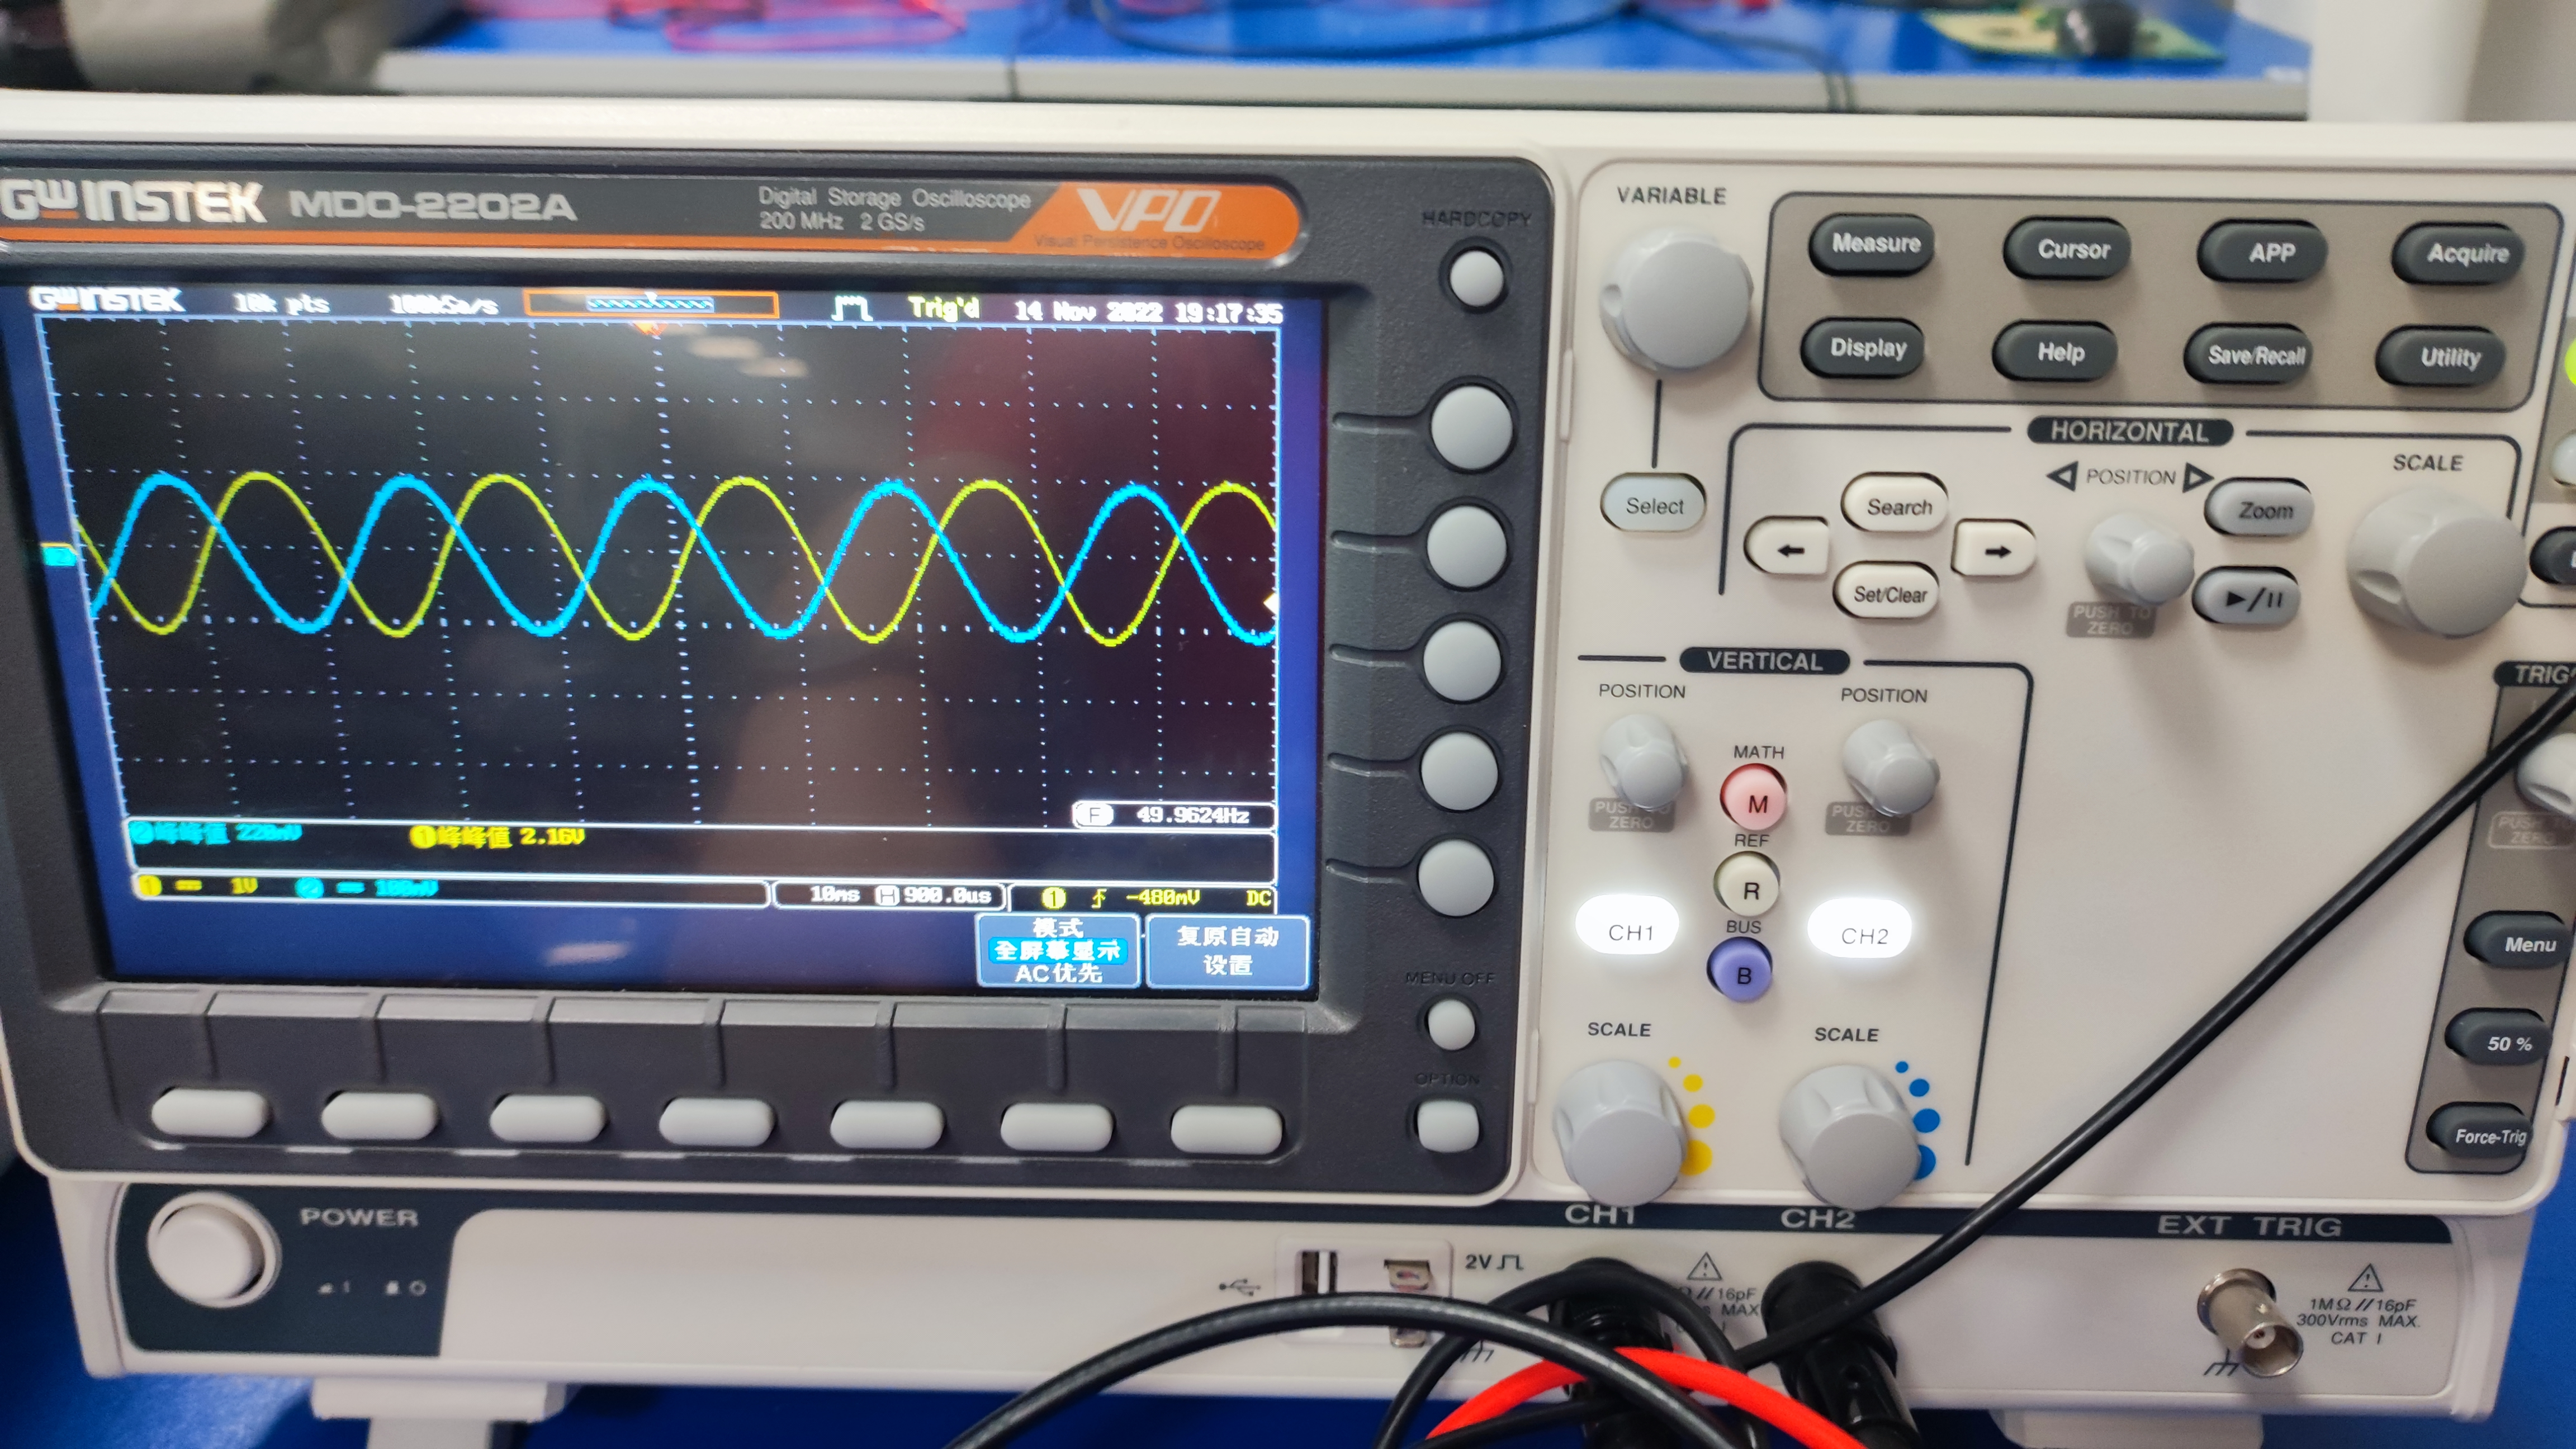
\includegraphics[width=0.9\linewidth]{图片/空载放大}
			\caption{负载放大示波器}
		\end{minipage}		
	\end{figure}

	\section{代替法测量输入电阻}
	运放工作在静态工作点, 当$K_1$端与$K_3$端相连, 测出$U_{K1}$, 断开$K_1$端与$K_3$端, 连接$K_1$端与$K_4$端, 调节$R_{W5}$使此时$U_{K1}$与刚才相等. 断开$K_4$端, 测量$R_{W5}$值, 即为等效输入电阻值. 测量得到的$R_{W5}$大小为$4.745k\Omega$. 
	
	$R_O=\left(\frac{U_O^{\prime}}{U_O}-1\right) \times R_L \text{. }  U_O^{\prime} \text { 为空载时输出,  } U_O \text { 为带负载时输出 }$. 计算得到的等效输出电阻大小为$4.63k\Omega$. 
	
	\section{电路调试练习}
	在电路正常放大的基础, 分别
	\subsection{将K3与K5用一根导线连接(电容被短路)}
	推测电容短路后, 静态工作点发生变化, 基极接地电阻变小, 输出放大图线发生失真现象. 如调试示波器图像中第一幅图所示. 
	\subsection{将K8与K9的连线断开}
	此时放大电路没有供电, 放大电路不工作, 输出波形消失, 如第二个图象所示. 
	\subsection{将K5与地连接(电阻被短路)}
	基极短路, $U_{BE}$小于导通电压, 三极管不工作, 输出为0, 如第三个图像所示.
	
	\begin{figure}[h]
		\begin{minipage}[t]{0.33\linewidth}
			\centering
			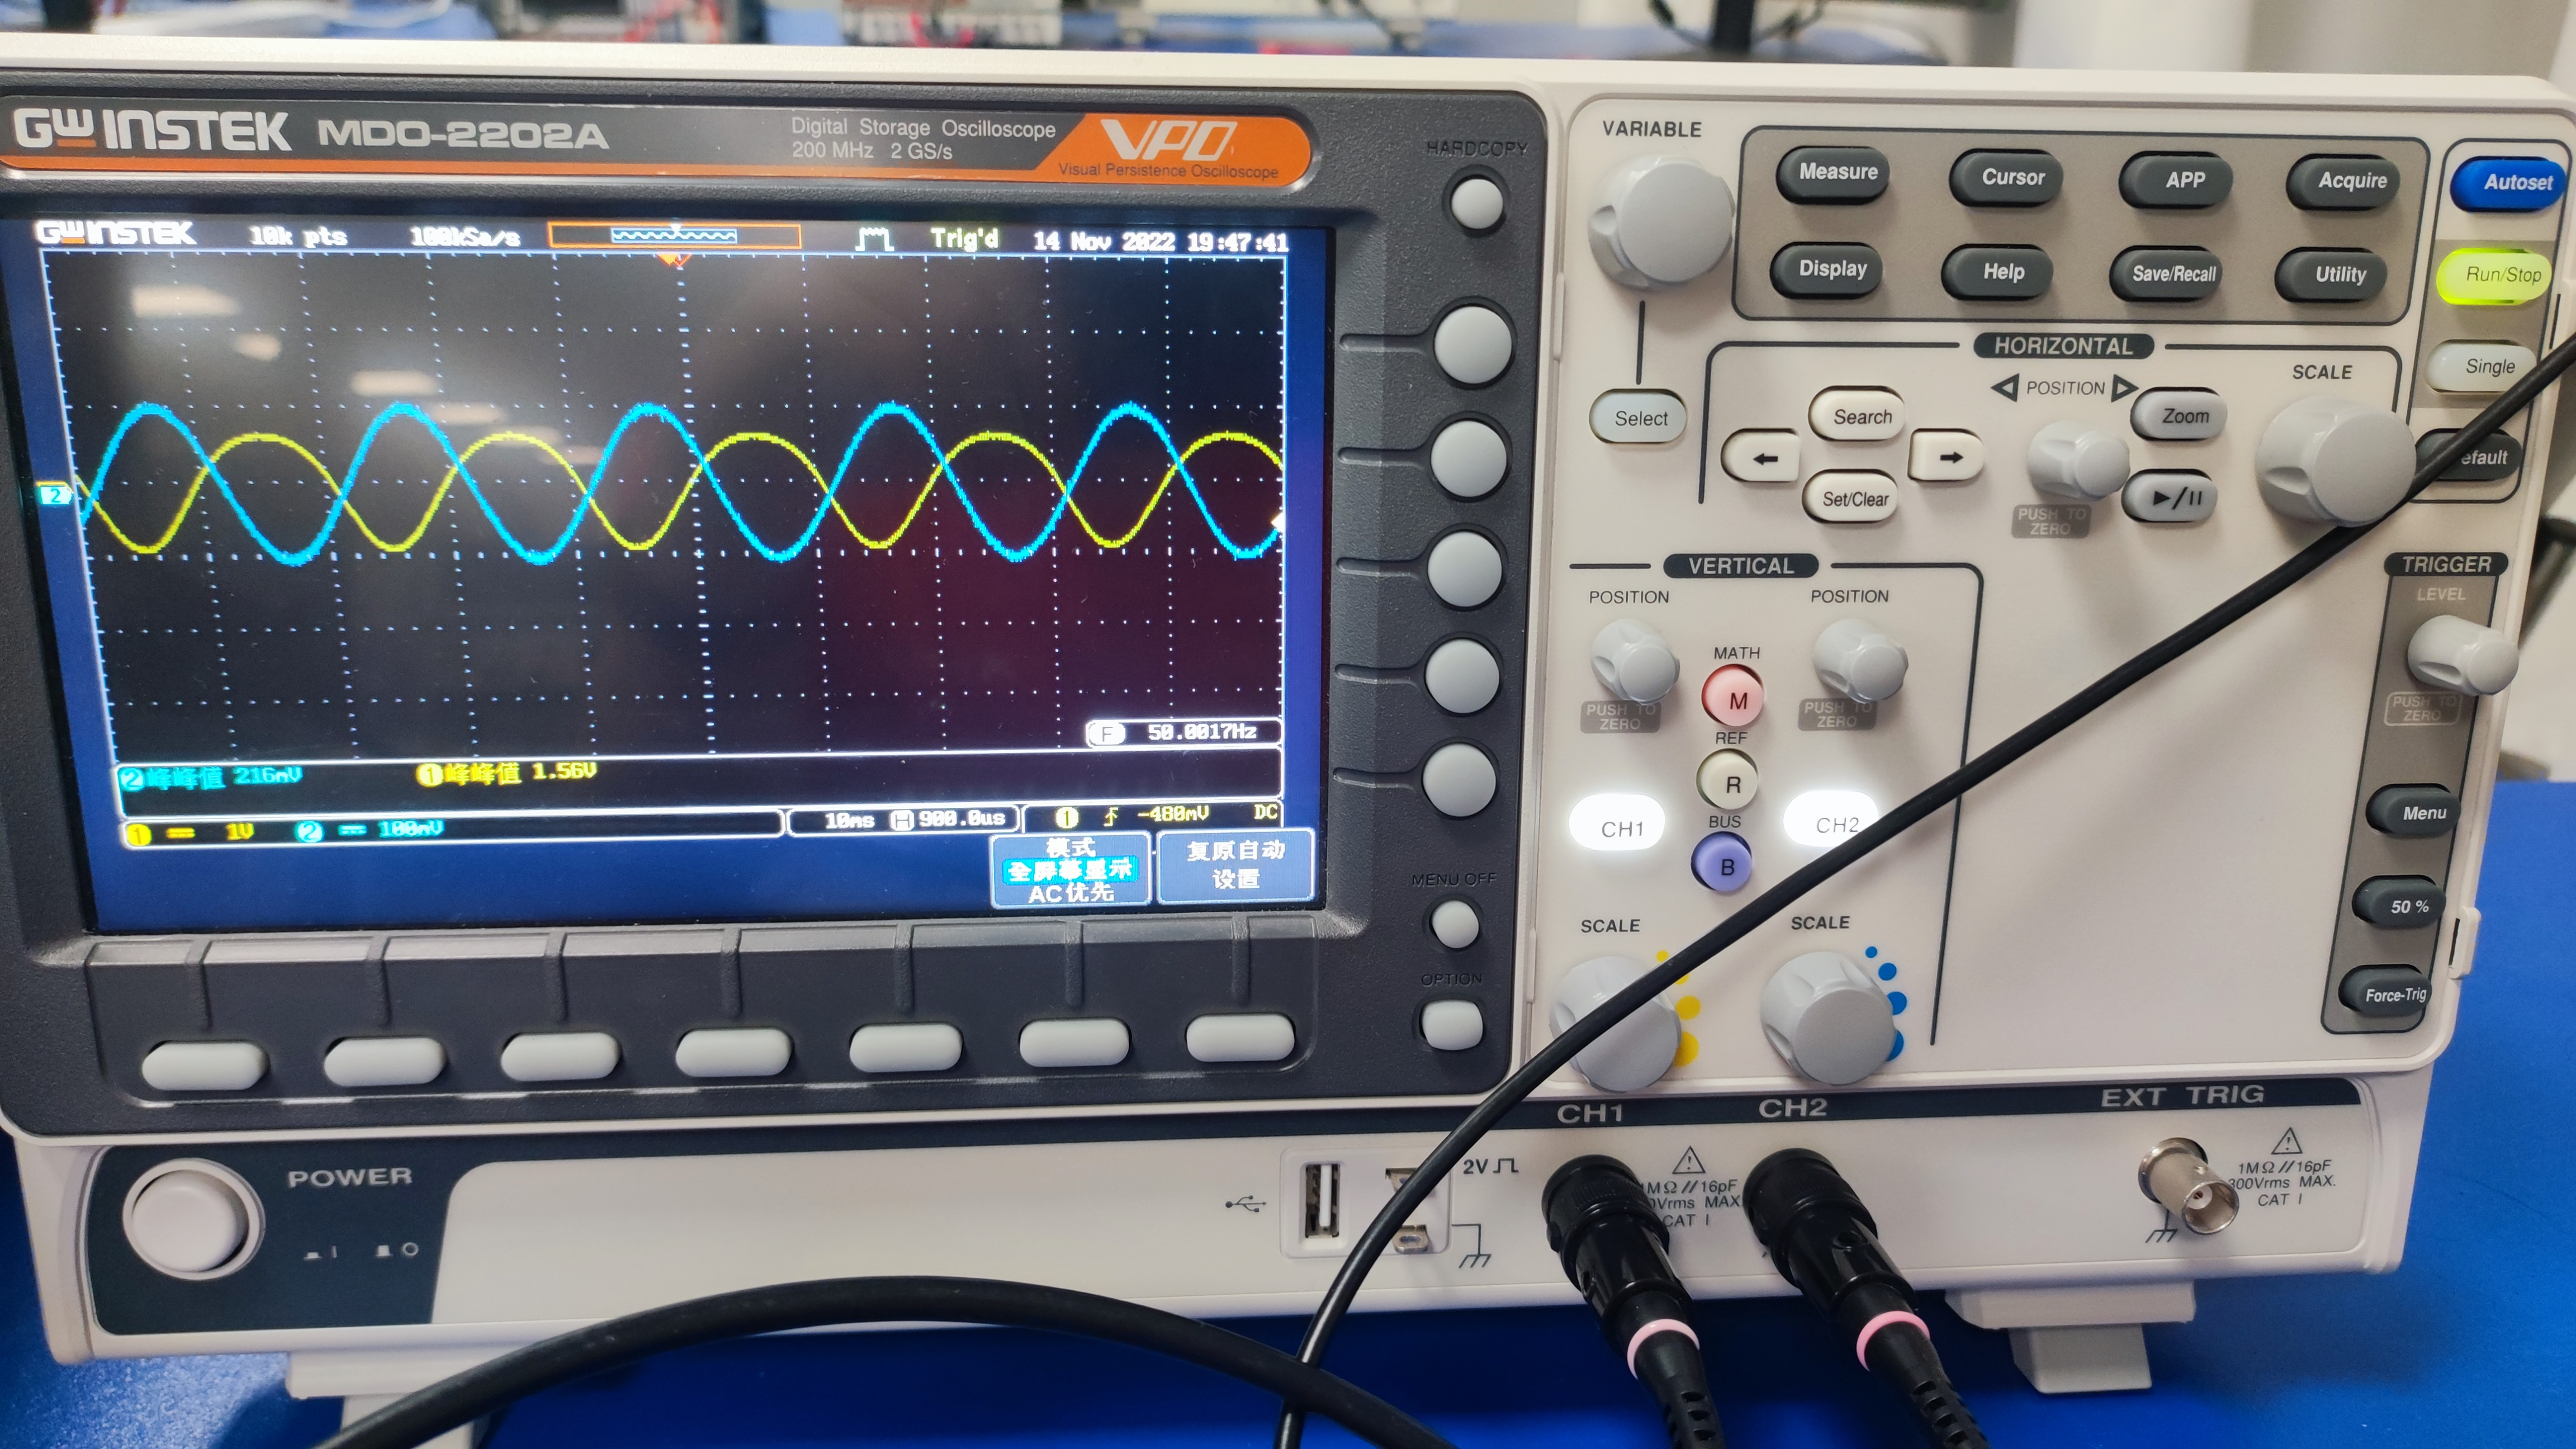
\includegraphics[width=0.9\linewidth]{图片/调试失真}
			\caption{失真图像}
		\end{minipage}
		\begin{minipage}[t]{0.33\linewidth}
			\centering
			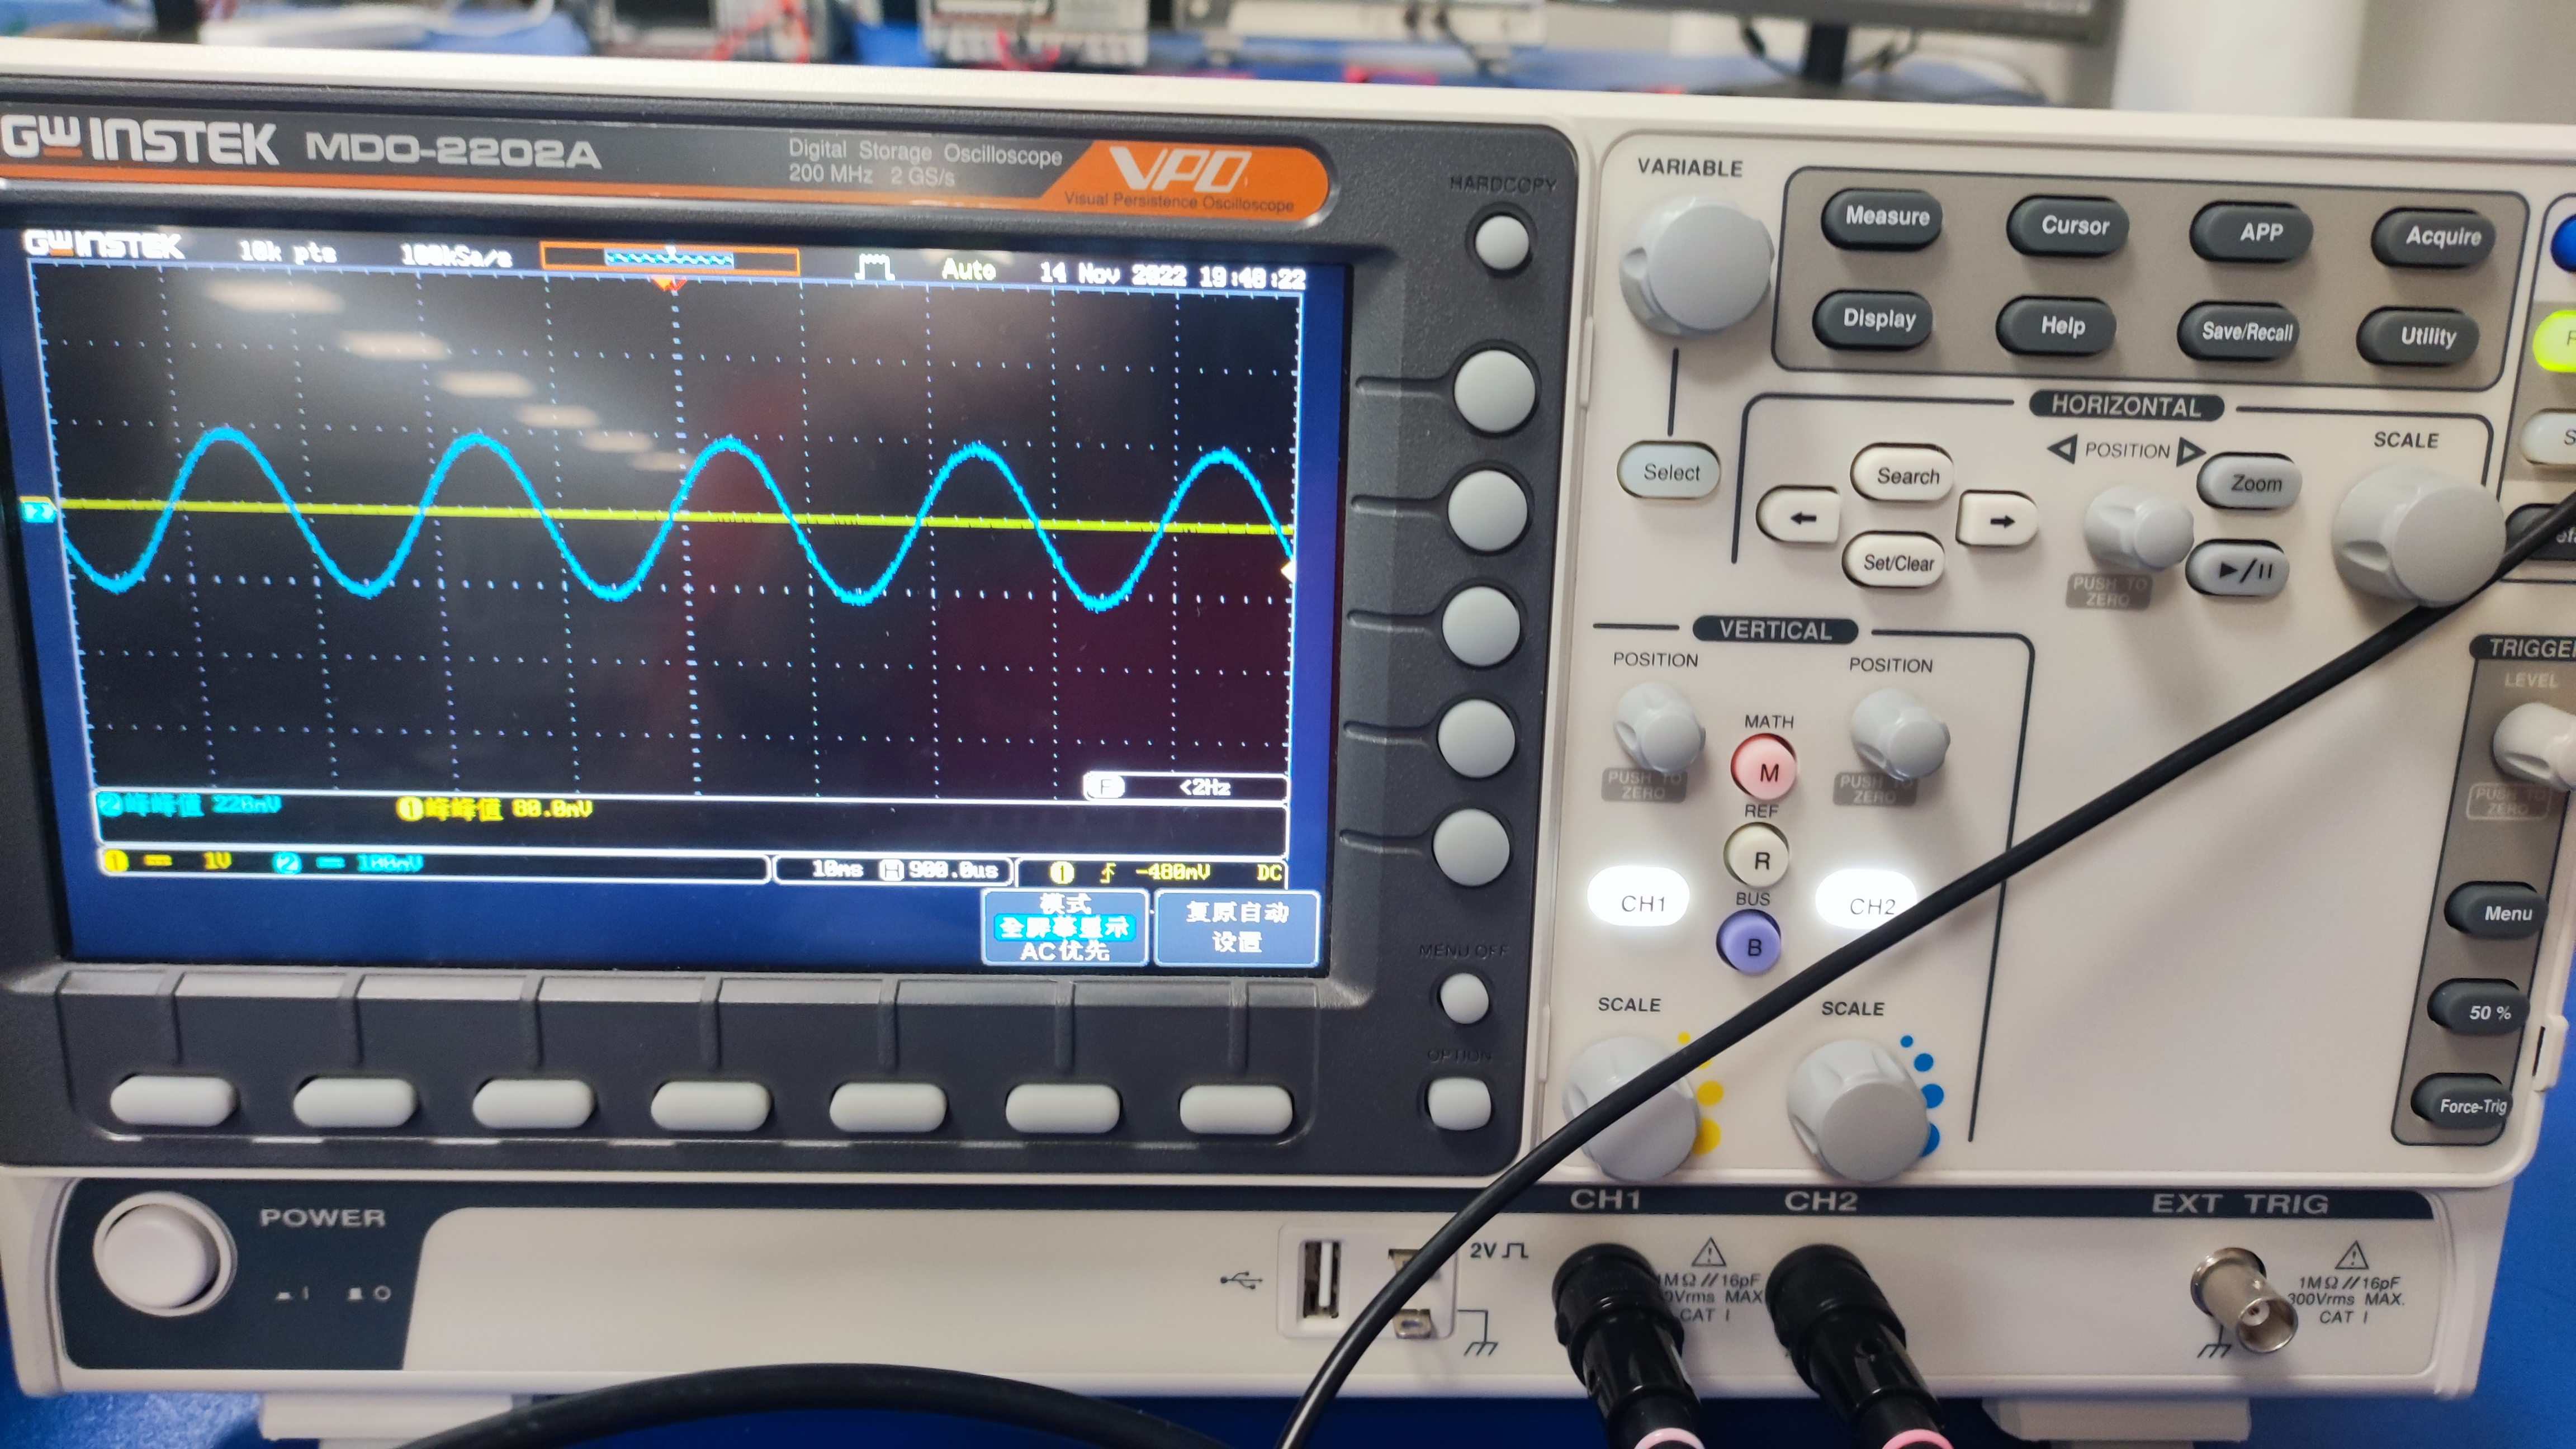
\includegraphics[width=0.9\linewidth]{图片/调试1}
			\caption{不工作图像1}
		\end{minipage}		
		\begin{minipage}[t]{0.33\linewidth}
			\centering
			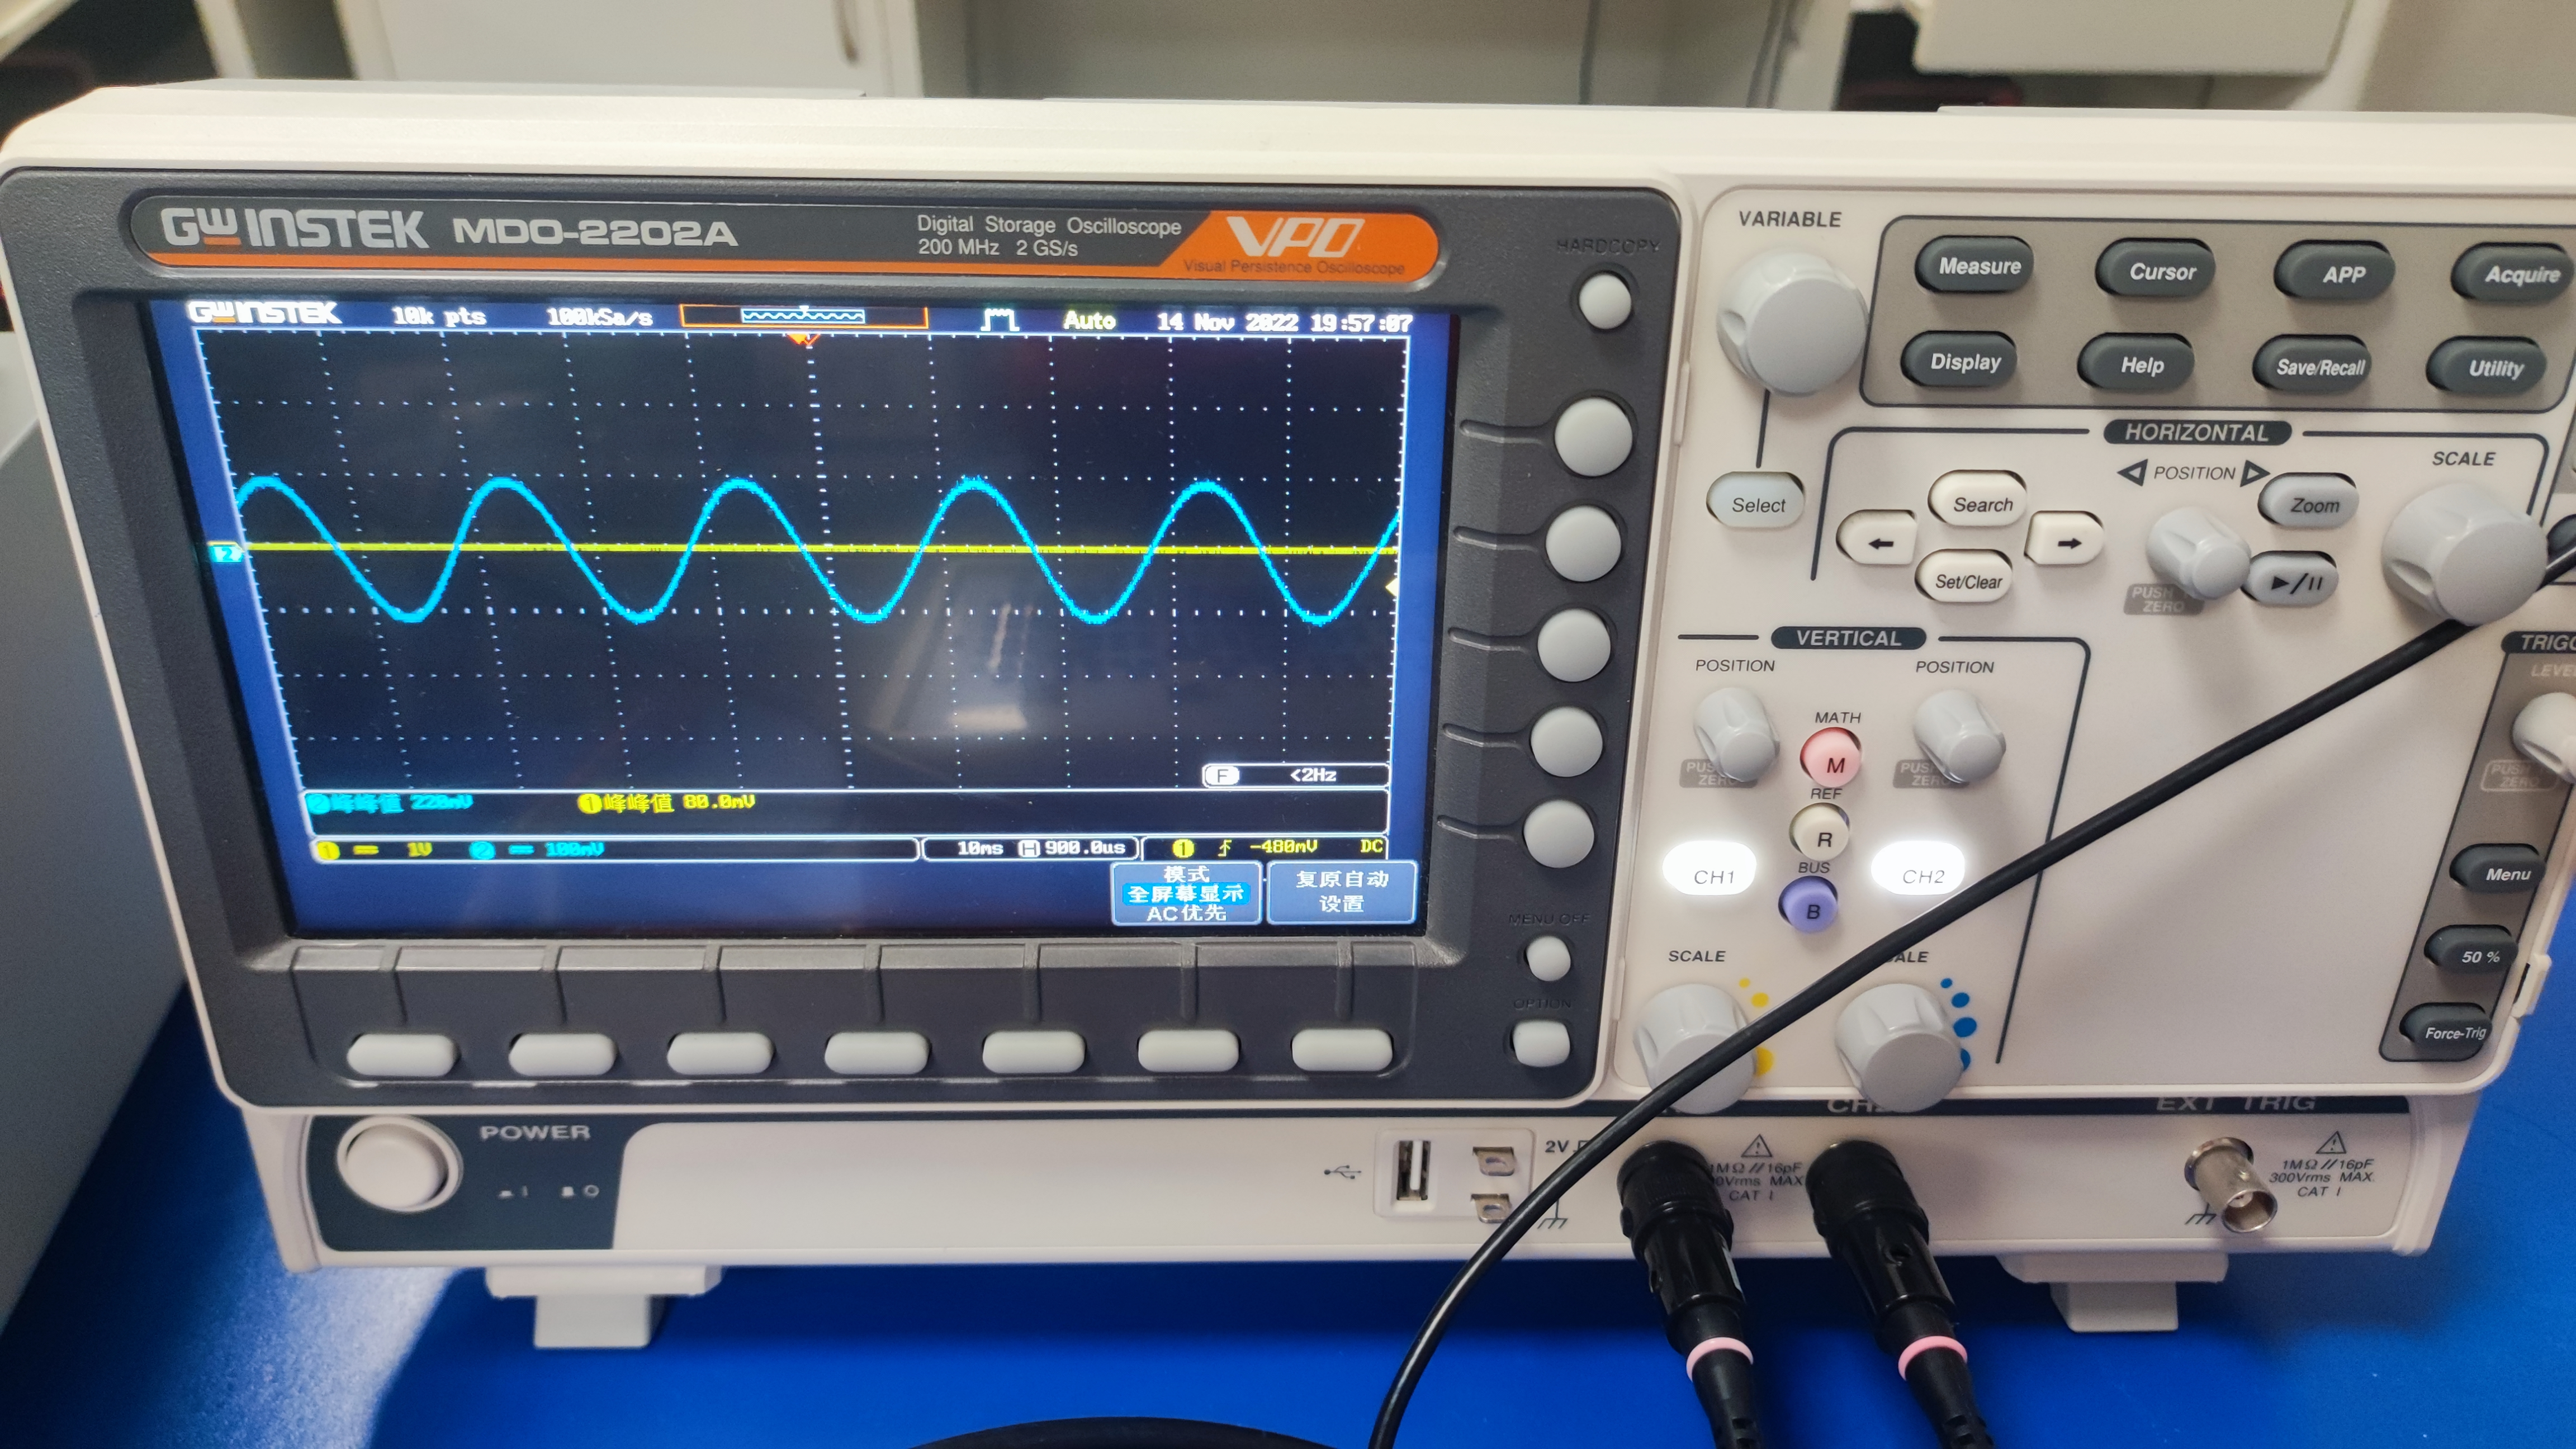
\includegraphics[width=0.9\linewidth]{图片/调试2}
			\caption{不工作图像2}
		\end{minipage}	
	\end{figure}
	
	调试电路接线如图. 
	
	\begin{figure}[h]
		\begin{minipage}[t]{0.5\linewidth}
			\centering
			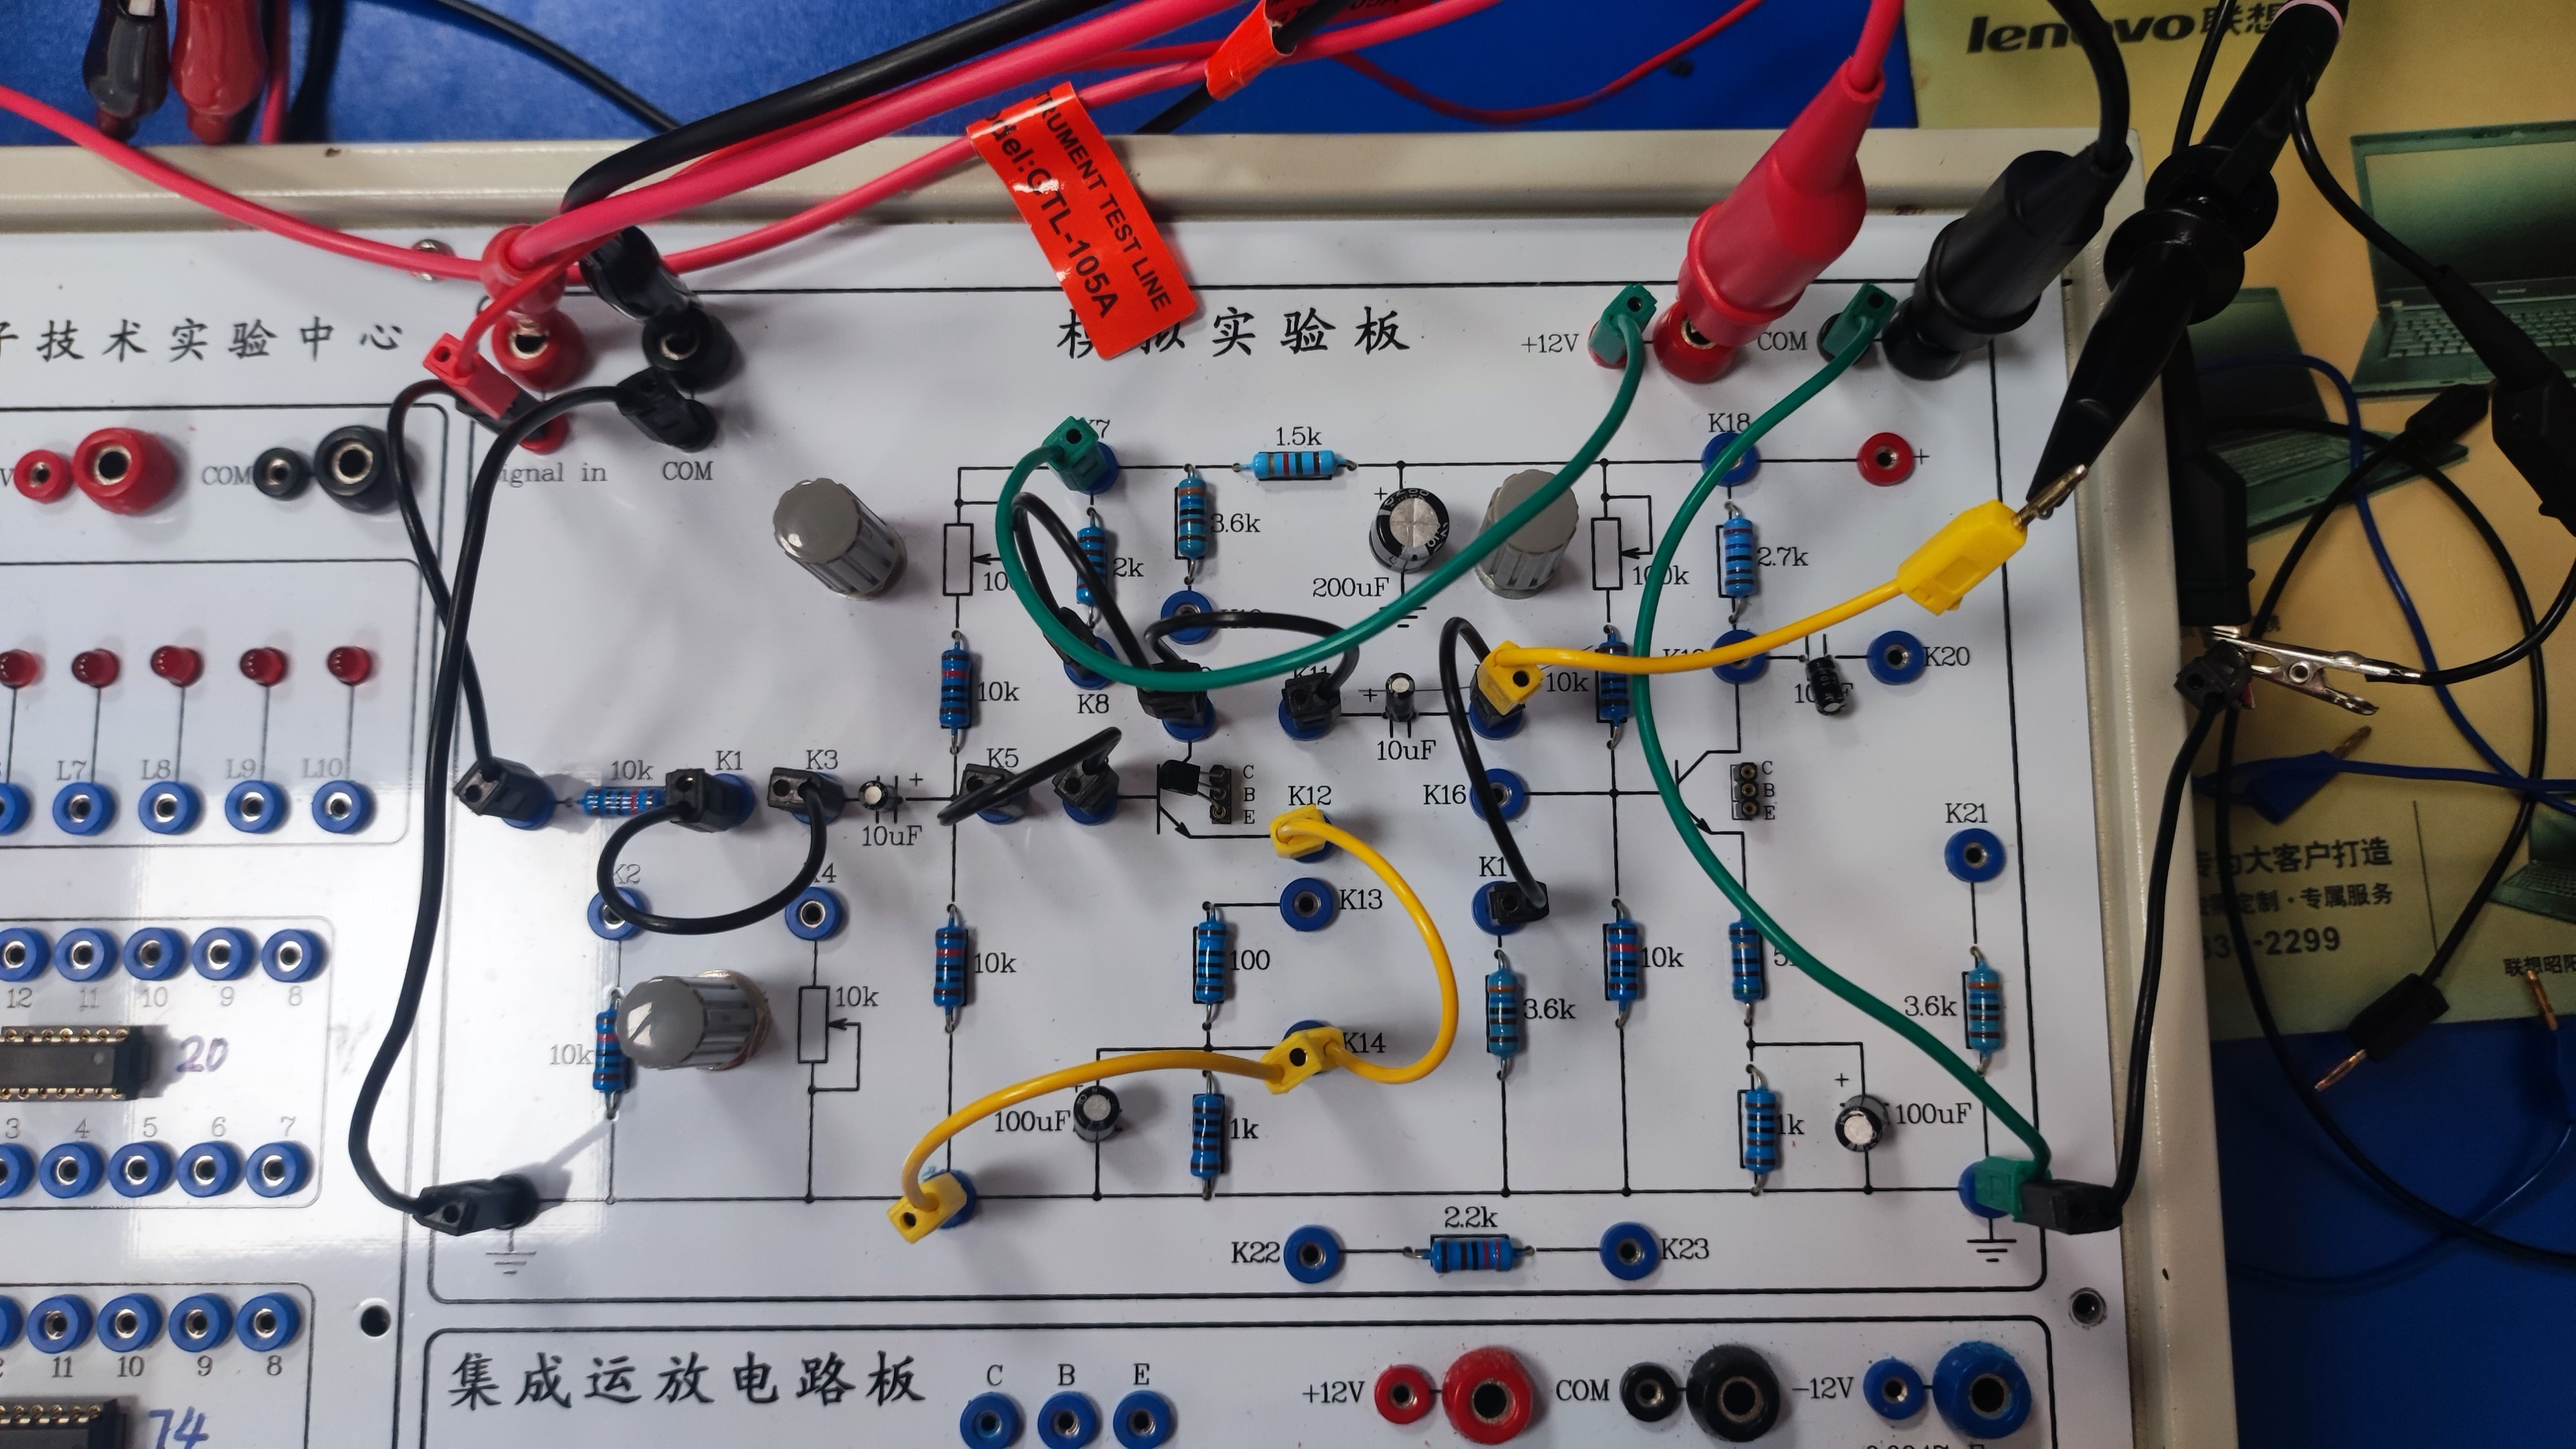
\includegraphics[width=0.9\linewidth]{图片/调试图1}
			\caption{故障1}
		\end{minipage}
		\begin{minipage}[t]{0.5\linewidth}
			\centering
			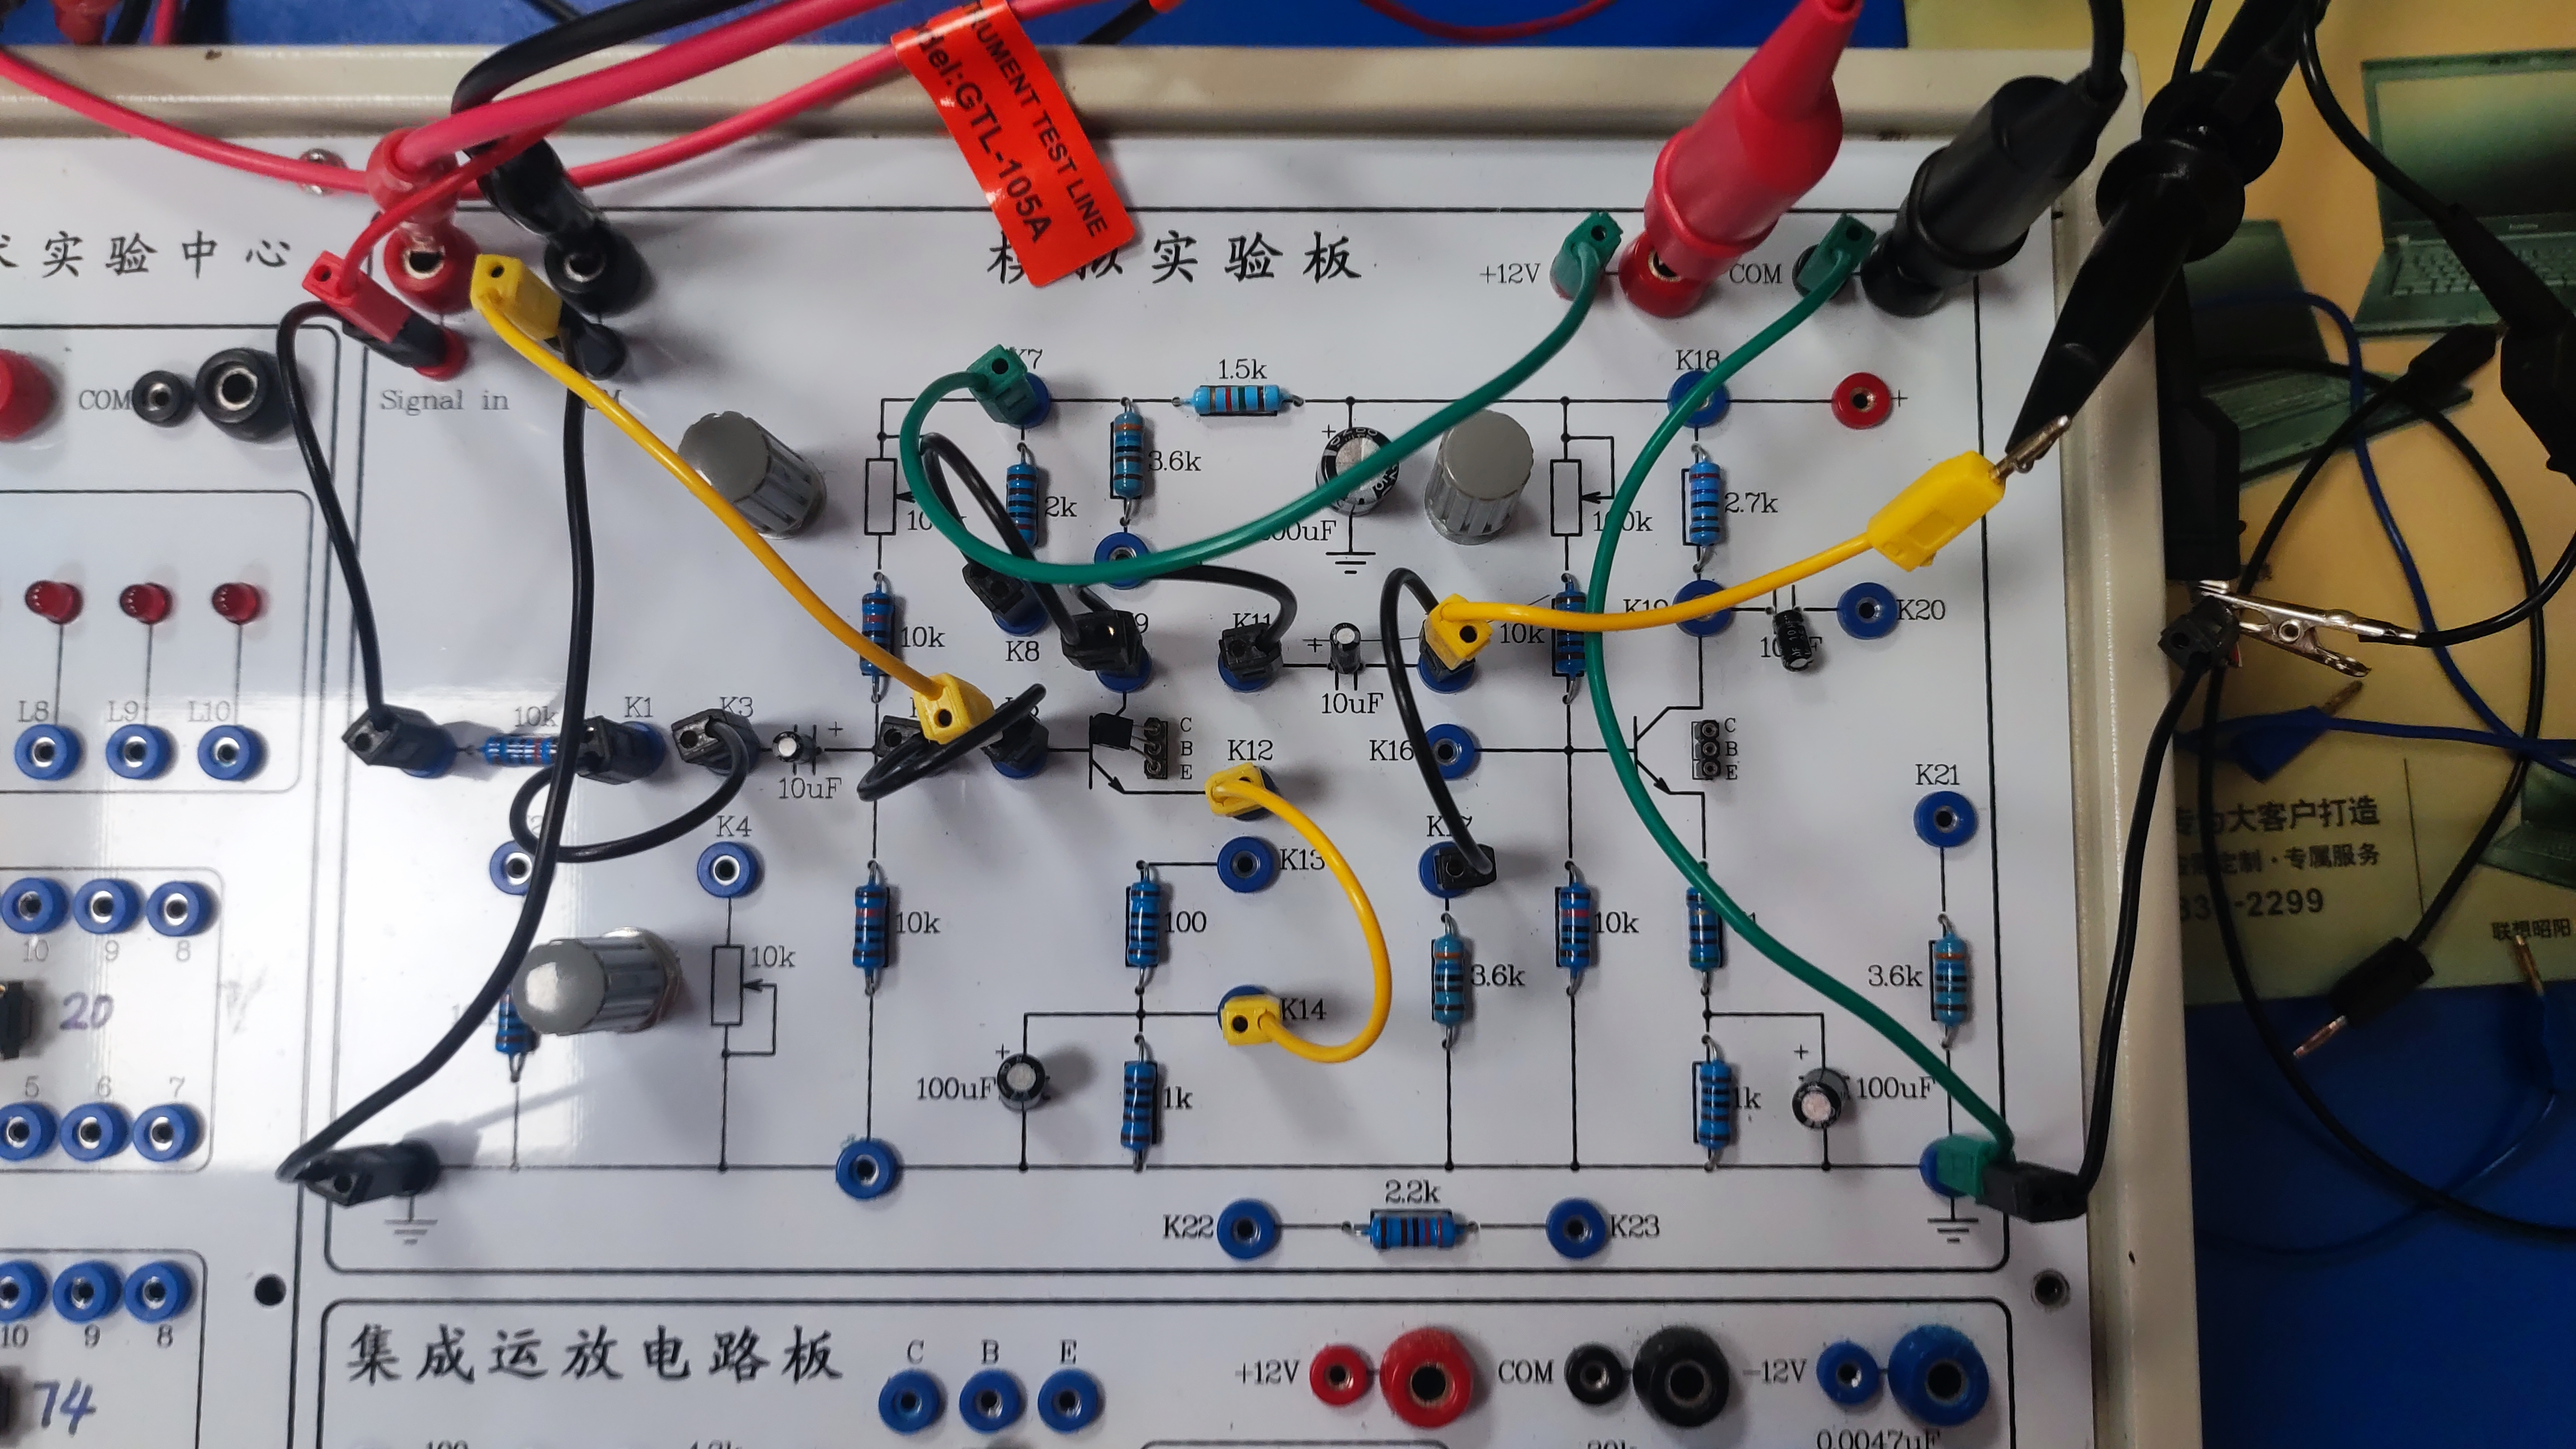
\includegraphics[width=0.9\linewidth]{图片/调试图2}
			\caption{故障2}
		\end{minipage}		
	\end{figure}

	\section{实验要点}
	\begin{enumerate}
		\item 使用万用表测量电压时注意交流档/直流档(档位用错测量结果无意义)
		\item 使用示波器观察波形时注意区分用DC耦合(看信号全貌)/AC耦合(只看信号的交流成分)
		\item 电容"通交阻直". 
	\end{enumerate}

	\section{实验总结}
	经过本次实验, 我对模拟电子技术的学习有了更深的理解, 对于三极管放大电路有了基本认识和使用经验. 
\end{document}